%-----------------------------------------------------------------------------
%
%               Template for sigplanconf LaTeX Class
%
% Name:         sigplanconf-template.tex
%
% Purpose:      A template for sigplanconf.cls, which is a LaTeX 2e class
%               file for SIGPLAN conference proceedings.
%
% Guide:        Refer to "Author's Guide to the ACM SIGPLAN Class,"
%               sigplanconf-guide.pdf
%
% Author:       Paul C. Anagnostopoulos
%               Windfall Software
%               978 371-2316
%               paul@windfall.com
%
% Created:      15 February 2005
%
%-----------------------------------------------------------------------------


%\documentclass[]{sigplanconf}

% The following \documentclass options may be useful:
%
% 10pt          To set in 10-point type instead of 9-point.
% 11pt          To set in 11-point type instead of 9-point.
% authoryear    To obtain author/year citation style instead of numeric.

%\usepackage{amsmath}

%\usepackage{graphicx}
%\usepackage{placeins} 
%\usepackage{url}
%\usepackage[T1]{fontenc}
%\usepackage{tikz}
%\usepackage{fancyvrb}

%\begin{document}

%\exclusivelicense
%\conferenceinfo{FHPC~'13}{September 23 2013, Boston, MA, USA} 
%\copyrightyear{2013} 
%\copyrightdata{978-1-4503-2381-9/13/09} 
%\doi{2502323.2502325}



%\titlebanner{DRAFT}        % These are ignored unless
%\preprintfooter{Counting Sort}   % 'preprint' option specified.

%\title{Efficient Counting Sort Implementations using an Embedded GPU Programming Language}
%\title{Implementing Counting Sort for GPUs using an Embedded Language}
%\title{Counting and Occurrence Sort for GPUs using an Embedded Language}
%\subtitle{Subtitle Text, if any}

%\authorinfo{Josef Svenningsson \and Bo Joel Svensson \and Mary Sheeran}
%           {Dept, of Computer Science and Engineering \\ 
%            Chalmers University of Technology}
%           {\{josefs, joels, ms\}@chalmers.se}

%\maketitle

\subsection*{Abstract}
This paper investigates two sorting algorithms: counting sort and a
variation, occurrence sort,  which also removes duplicate elements, 
and examines their suitability for running on the GPU. The duplicate 
removing variation
turns out to have a natural functional, data-parallel implementation
which makes it particularly interesting for GPUs.

The algorithms are implemented in Obsidian, a high-level domain
specific language for GPU programming.

Measurements show that our implementations in many cases outperform
the sorting algorithm provided by the library Thrust. Furthermore, occurrence
sort is another factor of two faster than
ordinary counting sort. We conclude that counting sort is an important
contender when considering sorting algorithms for the GPU, and that 
occurrence sort is highly preferable when applicable. We also show 
that Obsidian can produce very competitive code.


%% \category{CR-number}{subcategory}{third-level}
%% <<<<<<< HEAD

%% %% \terms
%% %% term1, term2

%% %% \keywords
%% %% keyword1, keyword2
%% \category{D.3.2}{Programming Languages}{Language Classifications}[Applicative (functional) languages; Concurrent, distributed, and parallel languages]
%% \category{D.3.4}{Programming Languages}{Processors}[Code generation]

%% %\terms
%% %term1, term2
%% \terms
%% Languages, Performance
%% =======
%\category{D.3.2}{Programming Languages}{Language Classifications}[Applicative (functional) languages; Concurrent, distributed, and parallel languages]
%\category{D.3.4}{Programming Languages}{Processors}[Code generation]
%% \terms
%% term1, term2
%% >>>>>>> 3b812338c4f7649982b17fb45df51f13d4285484

%\keywords
%keyword1, keyword2
%\keywords
%% <<<<<<< HEAD
%% Data parallelism, array programming, embedded language
%% =======
%Sorting, embedded language

%% >>>>>>> 3b812338c4f7649982b17fb45df51f13d4285484

\subsection{Introduction} 

Sorting is an ever important, ever fascinating field of computer
science. The introduction of GPUs has introduced new challenges in
designing fast sorting algorithms.

This paper focuses on counting sort together with a variation which
removes duplicate elements. We call this variation
{\em occurrence sort}. Counting sort is a non-comparing sort
suitable for parallel implementation. The occurrence sort variation 
presented here is interesting because it seems to be a particularly
good fit for executing on the GPU. It has a very natural functional,
data-parallel implementation. We believe we are the first to study
this variation in the literature.

These algorithms are explored in Obsidian \cite{JSLIC,PUSH}, a domain
specific language targeting GPU programming. The goal of Obsidian is
to strike a balance between high-level constructs and low-level control. 
We want to provide the programmer with a set of tools for low-level 
experimentation with the details that influence performance when 
implementing GPU kernels. The counting sort
case study shows that Obsidian generates competitive kernels with
relatively little programmer effort. That Obsidian is an embedded language 
allows us to rapidly experiment with the addition of features and with varying 
programming idioms. The version used in this case study
adds global arrays and atomic instructions to Obsidian, see section 
\ref{sec:OBSHist}. 

The contributions of this paper are:
\begin{itemize}
\item We provide measurements (section \ref{sec:CSORTBenchmarks}) showing
  that counting sort is a competitive algorithm for sorting keys on the GPU,
  outperforming the sorting implementation in the library
  Thrust\cite{THRUST} in many cases.
\item Occurrence sort is shown to be particularly
  suitable for implementing on the GPU (section \ref{sec:occur}) and
  performs well (section \ref{sec:CSORTBenchmarks}).
\item The Obsidian implementation of the two sorting algorithms is
  detailed along with the generated CUDA (sections
  \ref{sec:Obsidian} and \ref{sec:parallel}).
\end{itemize}


\subsubsection{Related work} 

Sorting has applications in the computer graphics field \cite{sintorn}. 
Example instances of sorting and duplicate element removal in computer graphics 
can be identified in references \cite{Olsson} and \cite{Karras}. Another example 
of where sorting and the removal of duplicates have applications is 
in databases \cite{REMOVEDUPS}. 

%% Sorting on the GPU is interesting both for computer graphics
%% applications \cite{SINTORN} and for using the GPU to offload the
%% processor, for example in database applications \cite{REMOVEDUPS}.

The paper \cite{CSORT} implements counting sort in CUDA, and also optimisations 
that overlap computations with transferring data to and from the GPU.
Our work differs by being implemented in a high-level embedded
language and also by implementation of the occurrence sort variant of counting sort. We have not been concerned with
trying to overlap computations and data transfer, but have instead
focused solely on computations within the GPU.

Obsidian is a high-level embedded language for GPU
programming. Other such approaches include Accelerate
\cite{Acc} and Nikola \cite{NIKOLA}. Accelerate and Nikola both take an even
higher level approach compared to Obsidian and abstract more from GPU
details. Another example of providing a high-level interface to
programming the GPU is the C++ library Thrust \cite{THRUST}.
%\cite{FELDSPAR} 

%% With the Obsidian language we raise the level of abstraction for 
%% GPU kernel implementation. In order to generate CUDA code that performs well, 
%% Obsidian tries to strike a balance between high level constructs and low level 
%% control. 

%% This paper describes a case study. We implement a sorting algorithm known 
%% as counting sort. As an extra bonus we explore a variant of counting sort 
%% that can be given a nice purely functional description and lends itself well 
%% to parallelisation. The experimental results in section \ref{sec:Benchmarks} 
%% compares the performance of the counting sort algorithm we implement here to 
%% the NVIDIA Thrust \cite{THRUST} library. The Obsidian generated kernels perform
%% very well at relatively light work effort. 

%% Counting sort places new demands on Obsidian and points out areas of 
%% improvement. Some left to do, some already implemented and used here. 
%% First, in order to implement counting sort we added atomic operations to 
%% Obsidian. However, currently you can only use them by very low level features 
%% of Obsidian. This is shown in section \ref{sec:parallel}. This paper also 
%% shows for the first time the new global arrays and what they can be used for.
   

%Vague intro ideas.
%\begin{itemize}
%  \item Quickly, what is our idea. 
%  \item Why is this sorting useful.
%        (Or is i just a fun experiment.) 
%  \item GPUs are pretty cool 
%  \item This is an Obsidian case-study. 
%  \item Sneak in ref to Feldspar.
%  
%\end{itemize} 

%\cite{CSORT} 
%\cite{FELDSPAR}

\subsection{Counting Sort}
\label{sec:algorithm}

Counting sort, like radix sort, relies on array indexing rather than
comparison to order elements. The key idea of counting sort is to
count the number of occurrences of each element, and then perform a
prefix sum over all the counts. The prefix sum generates an array
which, for each element in the original array, will point to its
position in the final sorted array. In order for this to work,
counting sort needs a lower and upper bound on the values of the
elements in the input array. Counting sort is typically explained in
terms of sorting integers and we will do the same here.

The array \verb!{5,2,5,7,1}! will be used as a running example. In
addition, the range \verb!(1,10)! will be the approximation of the
range of the keys in the input. A diagrammatic illustration of our
running example is presented in figure \ref{fig:example}.

\begin{figure}
\begin{small} 
\begin{verbatim}
countingSort :: (Int,Int) 
                -> Array Int Int 
                -> Array Int Int
countingSort range input =
  reconstruct $
  scanlArray (+) 0 $
  histogram range input

histogram :: (Int,Int) 
             -> Array Int Int 
             -> Array Int Int
histogram range = 
  accumArray (\i _ -> i+1) 0 range . elems . fmap dup

reconstruct :: Array Int Int -> Array Int Int
reconstruct arr = 
  array (0,arr!l-1)
    [ (a,i)
    | (i,e) <- init (assocs arr)
    , a <- [ e .. arr!(i+1) - 1] ]
  where (_,l) = bounds arr

dup a = (a,a)
\end{verbatim}
\end{small}
\caption{A Haskell specification of Counting Sort. The function
  \texttt{scanlArray} is not standard but works much like
  \texttt{scanl}
  for lists.}
\label{fig:haskell}
\end{figure}

%% \begin{figure}
%% \begin{center}
%% 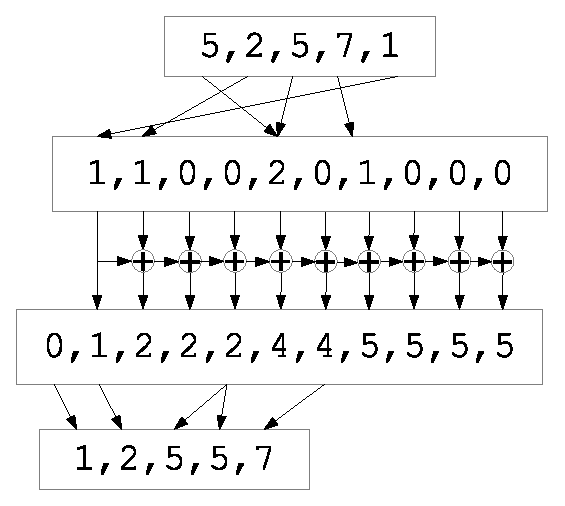
\includegraphics[height=4cm]{./CountingSortDiagram}
%% \end{center}
%% \caption{An example run of counting sort in diagrammatic form}
%% \label{fig:example}
%% \end{figure}
\begin{figure}

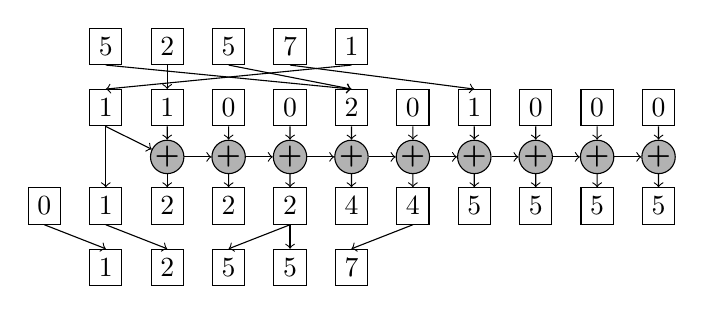
\begin{tikzpicture}[scale=0.78]
\usetikzlibrary{calc}
\tikzstyle{myedgestyle} = [->]
\tikzstyle{every node} = [draw, shape = rectangle]
 		 
\pgfmathsetmacro{\inpY}{1.5};
\pgfmathsetmacro{\vY}{\inpY-1};
\pgfmathsetmacro{\aY}{\vY-0.8};
\pgfmathsetmacro{\rY}{\aY-0.8};
\pgfmathsetmacro{\oY}{\rY-1};

\node (i0) at (1,\inpY) {$5$};
\node (i1) at (2,\inpY) {$2$};
\node (i2) at (3,\inpY) {$5$};
\node (i3) at (4,\inpY) {$7$};
\node (i4) at (5,\inpY) {$1$};

\node (v0) at (1,\vY) {$1$};
\node (v1) at (2,\vY) {$1$};
\node (v2) at (3,\vY) {$0$};
\node (v3) at (4,\vY) {$0$};
\node (v4) at (5,\vY) {$2$};
\node (v5) at (6,\vY) {$0$};
\node (v6) at (7,\vY) {$1$};
\node (v7) at (8,\vY) {$0$};
\node (v8) at (9,\vY) {$0$};
\node (v9) at (10,\vY) {$0$};

\draw [->] (i0.south) -- (v4.north);
\draw [->] (i1.south) -- (v1.north);
\draw [->] (i2.south) -- (v4.north);
\draw [->] (i3.south) -- (v6.north);
\draw [->] (i4.south) -- (v0.north);

\node (re) at (0,\rY) {$0$};
\node (r0) at (1,\rY) {$1$};
\node (r1) at (2,\rY) {$2$};
\node (r2) at (3,\rY) {$2$};
\node (r3) at (4,\rY) {$2$};
\node (r4) at (5,\rY) {$4$};
\node (r5) at (6,\rY) {$4$};
\node (r6) at (7,\rY) {$5$};
\node (r7) at (8,\rY) {$5$};
\node (r8) at (9,\rY) {$5$};
\node (r9) at (10,\rY) {$5$};


\tikzstyle{every node} = [draw, inner sep=0.1, fill=gray!60,shape = circle]

\node (1) at (2,\aY) {\bf{+}};
\node (2) at (3,\aY) {\bf{+}};
\node (3) at (4,\aY) {\bf{+}};
\node (4) at (5,\aY) {\bf{+}};
\node (5) at (6,\aY) {\bf{+}};
\node (6) at (7,\aY) {\bf{+}};
\node (7) at (8,\aY) {\bf{+}};
\node (8) at (9,\aY) {\bf{+}};
\node (9) at (10,\aY) {\bf{+}};


\foreach \i in {1,...,9}
{
	\draw [->] (v\i.south) -- (\i);
	\draw [->] (\i.south) -- (r\i);
}

\foreach \i in {1,...,8}
{
    \pgfmathtruncatemacro{\n}{(\i+1)};
    \draw [->] (\i) -- (\n);
}

\draw [->] (v0.south) -- (r0);
\draw [->] (v0.south) -- (1);

\tikzstyle{every node} = [draw, shape = rectangle]
\node (o0) at (1,\oY) {$1$};
\node (o1) at (2,\oY) {$2$};
\node (o2) at (3,\oY) {$5$};
\node (o3) at (4,\oY) {$5$};
\node (o4) at (5,\oY) {$7$};

\draw [->] (re.south) -- (o0.north);
\draw [->] (r0.south) -- (o1.north);
\draw [->] (r3.south) -- (o2.north);
\draw [->] (r3.south) -- (o3.north);
\draw [->] (r5.south) -- (o4.north);

\end{tikzpicture}

\caption{An example run of counting sort in diagrammatic form}
\label{fig:example}
\end{figure}
 
Counting sort consists of three steps: histogram creation, prefix sum
and reconstruction.

The histogram creation step computes a new array which records how
many times an integer occurs in the input array, i.e. the new array is
a histogram of the input array. The size and indices of the histogram
array are determined by the range which approximates the lower and
upper bounds of the keys.

Computing the histogram of \verb!{5,2,5,7,1}! with the range \verb!(1,10)!, 
results in \verb!{1,1,0,0,2,0,1,0,0,0}!.
%When running the example array \verb!{5,2,5,7,1}! through \\
%\verb!histogram! together with the range \verb!(1,10)! the resulting
%histogram is \verb!{1,1,0,0,2,0,1,0,0,0}!. 
Indexing in this array
starts at \verb!1! because that's the lower bound given in the
range. Each element in the histogram indicates how many times the
corresponding value occurs in the input array. For example, \verb!5!
occurs twice and \verb!8! occurs zero times.

The second step of the algorithm computes the prefix sum (or inclusive
scan with plus) of the histogram array, and prepends a zero.  For input array
\verb!{5,2,5,7,1}!  and range \verb!(1,10)!, the histogram array is
\verb!{1,1,0,0,2,0,1,0,0,0}! and its prefix sum is {\tt
  \{0,1,2,2,2,4,\allowbreak{}4,5,5,5,5\}}. 

%\verb!{0,1,2,2,2,4,4,5,5,5,5}!. This array starts with 0 and is one
%longer than the histogram array.

The array computed by the prefix sum is called the position array. It
indicates where in the final sorted array each value is placed. The
indices of the position array correspond to values in the final array
and the elements correspond to positions in the final array. The
reconstruct step takes care of distributing the values into the final
sorted array. For each index in the position array, the difference
between the element at that index and the index plus one is
computed. This difference indicates how many times the value occurs in
the final array.

The position array in our running example is {\tt\{0,1,2,2,2,4,\allowbreak{}4,5,5,5,5\}}.
Indexing starts at \verb!1! just as with the histogram. As an example,
element \verb!1! occurs once in the final array because the
difference between the element at position \verb!1! and \verb!2! in
the position array is precisely one. Also, \verb!1! is placed
on index \verb!0!. Furthermore, element \verb!5! occurs twice in
the final array (the difference between \verb!2! and \verb!4! in the
position array), on indices \verb!2! and \verb!3!. Continuing this
process with all elements will result in the following final array:
\verb!{1,2,5,5,7}!.

A functional description of counting sort can be found in figure
\ref{fig:haskell}. The main function is \verb!countingSort! which
takes two arguments: a range with a safe approximation of the lower
and upper bounds of the values in the input array, and the input array
itself. The histogram step is implemented by the function
\verb!histogram!, the prefix sum with \verb!scanlArray! and the
reconstruct step with the function \verb!reconstruct!.

\subsubsection{Occurrence sort: Removing duplicates}

There is an interesting variation of counting sort which removes
duplicate elements. It seems to be folklore; it is mentioned on
Wikipedia \cite{wikipedia}. However, we haven't found any description
of it in the literature. It is particularly interesting because it
allows for an efficient data-parallel implementation.
%% something which
%% will be explored in section \ref{sec:parallel}. Here we focus on the 
%% functional specification of the algorithm.
%% The rest of this
%% section will focus on the functional specification of the algorithm.


\begin{figure}
\begin{small}
\begin{verbatim}
countingSort :: (Int,Int) 
                -> Array Int Int 
                -> Array Int Int
countingSort range input =
  reconstruct $
  scanlArray (+) 0 $
  occurs range input

occurs :: (Int,Int) 
          -> Array Int Int 
          -> Array Int Int
occurs range = 
  accumArray (\_ _ -> 1) 0 range . elems . fmap dup
\end{verbatim}
\end{small}
\caption{A Haskell specification of occurrence sort}
\label{fig:duphaskell}
\end{figure}

Figure \ref{fig:duphaskell} shows the changes we make 
to counting sort in order to obtain occurrence sort.
%% counting sort compute a sorted array and at the same time remove
%% duplicate elements. 
Only the \verb!histogram! function needs changing
so that instead of computing an actual histogram which counts the
number of occurrences of an element, it only records if an element
occurs or not with a \verb!1! or a \verb!0!. Since the function
no longer computes a histogram it has been renamed to
\verb!occurs!.

The prefix sum and the reconstruction step can be kept intact. They
will still compute the correct result.

Compared to the full counting sort, occurrence sort has some
interesting properties which make it more suited for parallel execution.
In particular, the histogram construction phase and the reconstruction
phase allow for less synchronisation.

When constructing the histogram in the counting sort algorithm, an
index has to be incremented each time the corresponding value is found
in the input array. When parallelising this operation, it is important
that the increments are done atomically, which incurs a cost. The occurs
phase presented above doesn't need to employ any special mechanism to
ensure atomicity, since it writes a single word with the value $1$ to
memory.

Given the array \verb!{5,2,5,7,1}! as input and \verb!(1,10)!  as
range, the occurs step will now compute
\verb!{1,1,0,0,1,0,1,0,0,0}!. The prefix sum will in turn produce the
following position array: \verb!{0,1,2,2,2,3,3,4,4,4,4}!. The
reconstruct step computes \verb!{1,2,5,7}!. In particular,
there is only one occurrence of \verb!5! in the final array.

\subsection{Graphics Processing Units, accessible high performance parallel computing}
\label{sec:gpu}

In the development of microprocessors, the addition of new cores is now the
way forward, rather than the improvement of single thread performance.
Graphics processing units (GPUs) have moved from being specialised graphics
engines to being suitable to tackle applications with high computational
demands. For a recent survey of the hardware, programming methods and tools,
and successful applications, the reader is referred to~\cite{GPUComputing}.
Figure~\ref{fig:image}, taken from that paper, and due to NVIDIA, shows the
architecture of a modern GPU from NVIDIA. It contains 16 multiprocessors, 
grouped in pairs that share a texture fetch unit (TF in the figure). The 
texture fetch unit is of little importance when using the GPU for general 
purpose computations. Each multiprocessor has 8 stream processors (marked 
SP in the figure). These stream processors has access to 16kB of shared memory.  

See reference~\cite{GPUComputing} for information about
the very similar AMD GPU architecture. We have used the NVIDIA architecture,
but developments are similar at AMD. Intel's Larrabee processor points to a
future in which each individual core is considerably more powerful than in
today's GPUs~\cite{IntelLarrabee}.

%along with shared data and instruction caches, and 16kB of shared memory. 

The question of how to program powerful data-parallel processors is likely
to continue to be an interesting one. Unlike for current multicore machines,
the question here is how to keep a large number of small processors
productively occupied. NVIDIA's solution has been to develop the
architecture and the programming model in parallel. The result is called
CUDA -- an extension of C designed to allow developers to exploit the power
of GPUs. Reference~\cite{GPUCudaLuebke} gives a very brief but illuminating
introduction to CUDA for potential new users. The idea is that the user
writes small blocks of straightforward C code, which should then run in
thousands or millions of threads. We borrow the example from the above
introduction. To add two $N \times N$ matrices on a CPU, using C, one would
write something like

\begin{code}
// add 2 matrices on the CPU:
void addMatrix(float *a, float *b, float *c, int N)
{
  int i, j, index;
  for (i = 0; i < N; i++) {
    for (j = 0; j < N; j++) {
      index = i + j * N;
      c[index]=a[index] + b[index];
    }
  }
}
\end{code}
\FloatBarrier

\begin{figure}%
\begin{center}
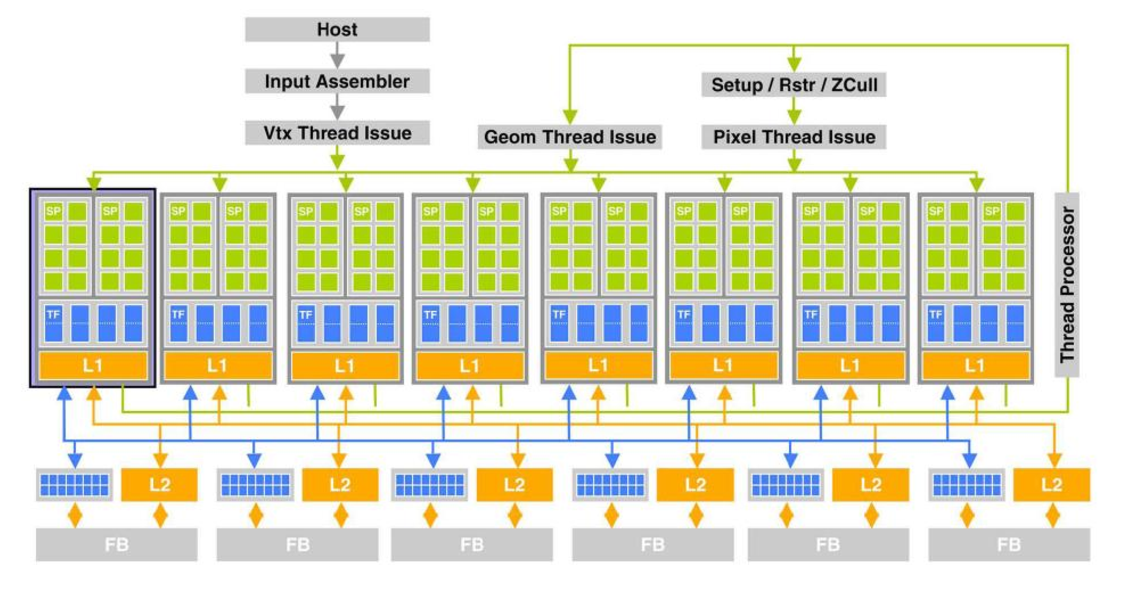
\includegraphics[height = 6cm]{./ifl/image_top.pdf}
%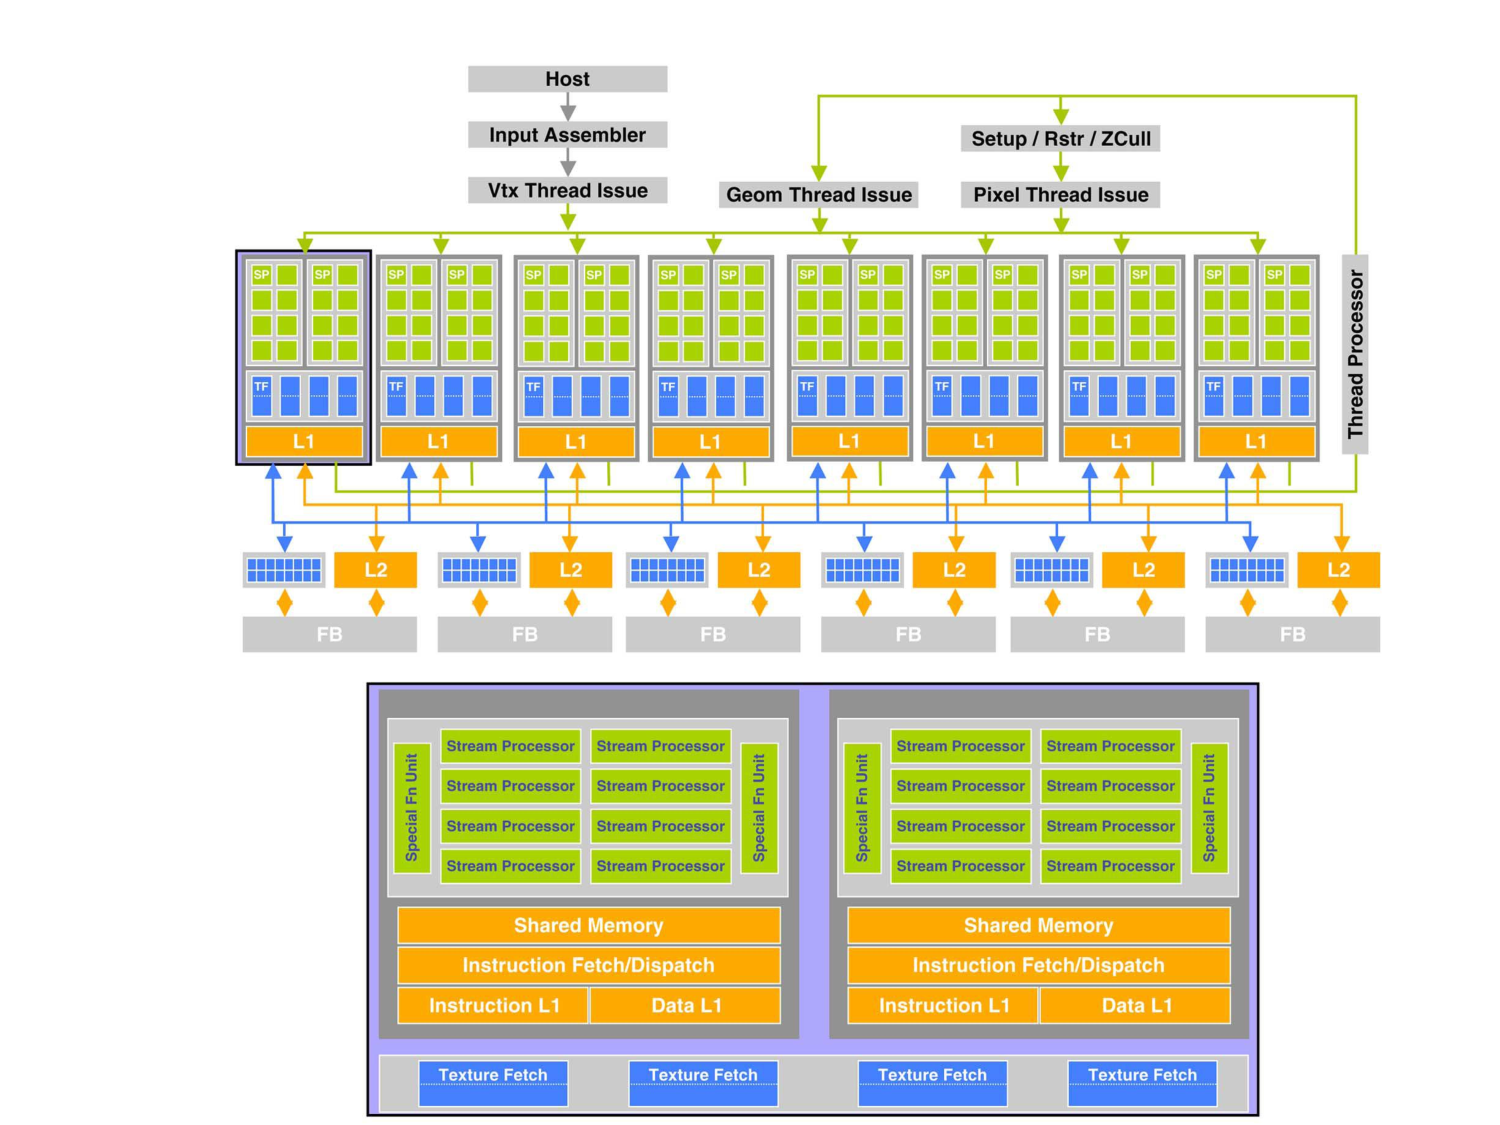
\includegraphics[width = 14cm]{image.pdf}
\caption{The NVIDIA 8800GTX GPU architecture, with 8 pairs of multiprocessors. Diagram courtesy of NVIDIA.}\label{fig:image}
\end{center}
\end{figure}


\noindent In CUDA, one writes a similar C function, called a {\em kernel},
to compute one element of the matrix. Then, the kernel is invoked as many
times as the matrix has elements, resulting in many threads, which can be
run in parallel. A predefined structure called {\tt threadIdx} is used to
label each of these many threads, and can be referred to in the kernel.
\begin{code}
// add 2 matrices on the GPU (simplified)
__global__ void addMatrix(float *a,float *b, float *c, int N)
{
  int i= threadIdx.x;
  int j= threadIdx.y;
  int index= i + j * N;
  c[index]= a[index] + b[index];
}

void main()
{
  // run addMatrix in 1 block of NxN threads:
  dim3 blocksize(N, N),
  addMatrix<<<1, blocksize>>>(a, b, c, N);
}
\end{code}
Here, a two dimensional {\em thread block} of size $N \times N$ is created.

CUDA uses {\em barrier synchronisation} and {\em shared memory} for
introducing communication between threads. Contents of shared memory (16kB
per multiprocessor in the architecture shown in Figure~\ref{fig:image}) is
visible to all threads in a thread block. It is very much faster to access
this shared memory than to access the global device memory. We shall see
later that Obsidian provides users with both shared and global arrays,
giving the user control over where data is to be stored.

Since many threads are now writing and reading from the same shared memory,
it is necessary to have a mechanism that enables the necessary
synchronisation between threads. CUDA provides a barrier synchronisation
mechanism called {\tt \_\_syncthreads()}. Only when all threads in a block
have reached this barrier can any of them proceed. This allows the
programmer to ensure safe access to the shared memory for the many threads
in a thread block.

Now, a {\em grid} is a collection of thread blocks. Each thread block runs
on a single multiprocessor, and the CUDA system can schedule these individual
blocks in order to maximise the use of GPU resources. A complete program
then consists not only of the kernel definitions, but also of code, to be
run on the CPU, to launch a kernel on the GPU, examine the results and
possibly launch new kernels. In this paper, we will not go into details
about how kernels are coordinated, but will concentrate on how to write
individual kernels, as this is the part of Obsidian that is most developed.
In Obsidian, we write code that looks like the Lava descriptions in
section~\ref{sec:combinators}, and we generate CUDA code like that shown
above. This is a considerably more complex process than the generation of
netlists in Lava.



\section{Obsidian} 
\label{sec:Obsidian} 
%\FloatBarrier

Obsidian is a programming language for expressing general purpose 
GPU kernels, compute kernels, in a high level and functional style.  
Obsidian is embedded in Haskell.
Specifically, Obsidian is a library of functions for generating 
and combining abstract syntax trees.
%That Obsidian is embedded in Haskell means that it is a library of 
%functions for generating and combining abstract syntax trees. 
By using features of Haskell such as overloading and higher-order-functions, 
the library/language border is blurred and we call the result an embedded 
language. From the abstract syntax trees generated while running an 
Obsidian program, NVIDIA CUDA code is generated. 


\subsection{A brief history of Obsidian} 
\label{sec:OBSHist}

In the Obsidian project we experiment with combinators and language 
features for GPU kernel implementation. We seek to strike a balance 
between low-level control and useful high-level abstractions. Over time, this 
has led to a number of different versions of Obsidian. In reference \cite{JSLIC}, 
two versions of Obsidian differing by having a {\em monadic} or a limited {\em arrow} 
like interface are described. We have settled on using the monadic style. 

One of the array representations that Obsidian uses, the Pull array, was present already 
in the earlier work but went under a different name. It was not until discovering 
a complementary array representation, that we call push arrays, that the traditional 
array was renamed to pull. 

The Obsidian implementation of pull arrays was influenced by Pan's representation 
of images as functions from coordinates to colour values \cite{ELLIJFP}. A pull array 
is a function from index to value and an associated length.  

Push arrays were added to Obsidian first in reference \cite{PUSH}. A push array
specifies where elements are to end up in a result array, rather than where 
they come from (as in a pull array). In essence, a push array is a
computation which writes an array to memory, but is parameterised on
the {\em write function} which writes a single element into memory.
The push array function can then 
use the write function zero, one, or several times. 

Push arrays were added to Obsidian with the purpose of solving some performance 
issues that we had been struggling with for a long time. These problems were 
mainly concerned with concatenating or combining arrays in an efficient way.
Push arrays have also been adopted by others and are used in the implementation 
of filters in reference~\cite{FPCDSL} and in the new Nikola\footnote{github.com/mainland/nikola/blob/master/src/Data/Array/Nikola/Repr/Push.hs}.

Both push and pull arrays are virtual, in the sense that they do not directly 
correspond to any data in a region of memory. This virtual nature of the array 
representations gives us fusion of operations for free. The programmer has 
to explicitly force an array (using a {\tt force} function) to actually compute 
the values and store them in memory and to prevent operations from fusing. 

In the version of Obsidian used in this paper\footnote{github.com/svenssonjoel/Obsidian/branches/February2013}, new features were added.  We 
introduce two new variants of push and pull arrays called {\tt GlobPush} and 
{\tt GlobPull}. This introduces a distinction between local arrays, short 
enough to be computed by a block of the GPU, and global arrays that represent 
computations spread over blocks of the GPU. This is an important step when 
it comes to Obsidian's capabilities; we can now express in what order a kernel
fetches elements from global memory. 
Earlier versions of Obsidian were limited to straight-line block indexing. A kernel 
generated by older Obsidian accessed blocks of elements in a fixed way (thread block 
i accessed elements using {\tt (i * blocksize) + f tid}, where {\tt f} can permute 
indices within a block but there is no similar way to permute the actual blocks). 

In order to implement histograms we also need to add  atomic operations to the language. The addition of atomic operations here is 
done in a rather ad hoc way and pushes us to program in a very low-level and 
imperative style. We strive to incorporate much of CUDA's low-level functionality 
into Obsidian and adding atomic operations is an attempt in that 
direction.  

The version of Obsidian used in this paper also introduces a new monadic representation 
of GPU programs. We call the monad {\tt Program}. The {\tt Program} type has a 
parameter that represents at what level in the GPU hierarchy it executes. There 
are sequential {\em Thread} programs and parallel {\em Block} and {\em Grid} programs. Type synonyms 
are available, {\tt TProgram}, {\tt BProgram} and {\tt GProgram}.   

Many of the new features we mention above have been further refined and 
are present in versions of Obsidian following the one we use in this paper. For 
example, in the master branch of Obsidian\footnote{github.com/svenssonjoel/Obsidian} we build on the ideas in this paper. 
There, global and local arrays are represented by the same data type. That 
work also goes further by implementing hierarchy generic functions that are 
applicable at different levels of the Thread, Block and Grid hierarchy. 
We are also experimenting with the addition of mutable arrays in order to 
better integrate the atomic operations\footnote{github.com/svenssonjoel/Obsidian/tree/mutable}. 




%% Obsidian raises the level of abstraction for GPU programming but wants 
%% to keep low level control. To facilitate this, Obsidian supplies different 
%% kinds of arrays. There are {\tt Push} and {\tt Pull} arrays for local 
%% computations and in the current version of 
%% Obsidian\footnote{github.com/SvenssonJoel/Obsidian} we add global arrays 
%% of types {\tt GlobPush} and {\tt GlobPull} to the language.

%% Both push and pull arrays are in some sense virtual. They do not necessarily 
%% represent data that exists in memory. Instead, the push and pull arrays 
%% represent ways to compute an array. Concretely, a pull array is function from 
%% index to element. A push array is a function that when given a write-function 
%% (a function that takes an index and an element to a program 
%% that represents the writing of that element into an array) gives 
%% a program that represents writing a number of elements. In 
%% Obsidian, there are three kinds of programs, represented by a {\tt Program} data 
%% type. TPrograms, BPrograms and GPrograms represent what a thread, block of 
%% threads and a grid of blocks can do. Thread programs are the result type in 
%% the so-called write-functions. BPrograms operate on local arrays and 
%% grid programs operate on global arrays. 
%% Since push and pull arrays are virtual operations upon them are fused 
%% automatically. The standard example is map-fusion {\tt (map a . map b = map (a . b))}. 
%% The programmer decides when, and if, intermediate values are computed and 
%% stored in memory by using a {\tt force} function.
%% %In order to ensure that an intermediate value is computed there is a {\tt force}
%% %function. 
%% The {\tt force} function takes a push or pull array and gives 
%% a block program resulting in a pull array. The block program writes the data 
%% contained in the array into shared memory and the return array symbolises 
%% reading from that memory. 
  
%% %Hence, when working with local push and 
%% %pull arrays the associated programs are thread and block programs and when 
%% %working with global arrays the grid programs also come into play.  

%% The push and pull arrays have different strengths. Pull arrays 
%% make it easy to implement functions such as {\tt map} and {\tt zipWith}. 
%% % and 
%% %also give map-fusion for free. A pull array is also easy to parallelise;  
%% %thread $i$ is in charge of computing element $i$.  
%% %The push arrays provide ways to compute arrays in a way so that thread $i$ 
%% %computes other elements than $i$. Actually, any thread be in charge of the 
%% %computation of any element of the result. 
%% Push arrays allow thread $i$ to compute array elements at indices other 
%% than $i$; this enables efficient array concatenation as well 
%% as the data scattering operations used later. For more information about 
%% push arrays, see reference \cite{PUSH}. 

%Both push and pull arrays are easy to parallelise. 
 
%In the current version of Obsidian\footnote{github.com/SvenssonJoel/Obsidian} 
%we are exploring ways to increase the scope of what kinds of compute kernels 
%we can describe and obtain efficient code for. One aspect of this exploration 
%is the addition of a new kind of array representation that we call 
%{\em push} arrays \cite{PUSH}. Previous versions of Obsidian 
%(described in \cite{JSLIC}) represented arrays as functions 
%from indices to values,we call these {\em pull} arrays. Another addition 
%is global arrays. Earlier versions of Obsidian has been focused on 
%expressing the kind of computations that takes place locally, in a block.  
 
%The pull representation of arrays make it easy to describe 
%functions that take arrays apart and gives fusion of operations (for 
%example map-fusion) for free. However, Combining arrays, such as the 
%array concatenate operation, is not efficient using this array 
%representation. We have had problems in generating good CUDA code 
%for such functions. For example concatenation of pull arrays 
%leads to conditionals in the generated code of a kind that can have 
%negative performance impact on the GPUs we are targeting. 
%The implementation of the algorithm described in this paper 
%uses both the pull and the push arrays offered by Obsidian. 

%The GPUs targeted by Obsidian has an hierarchical structure 
%in more senses than just its memory system. Threads are only 
%allowed to communicate using local shared memory in small groups 
%(thread blocks). 
%To match the hierarchal architecture of GPUs, Obsidian has local arrays 
%of type {\tt Pull a} and {\tt Push a}. These local arrays are used in the 
%implementation of programs that can be run by a block, in Obsidian these 
%programs are represented by a data type called {\tt BProgram}. There 
%are also global arrays types {\tt GlobPull a} and {\tt GlobPush a} that 
%are used in the implementation of programs executed by more than one MP, 
%these programs are represented by a {\tt GProgram} data type.   
%and global arrays of 
%types {\tt GlobPull a} and {\tt GlobPush a}.
%Global arrays are used when simple permutations of a large input array is 
%needed. Here it is important to that no communication needing 
%synchronisations occurs. Global arrays are also used as the inputs 
%and outputs of a top level Obsidian program (a program you want to generate runnable CUDA code from). In the cases where threads need to cooperate 
%on solving a task the local arrays should be used. 
\subsection{Obsidian programming example} 
\label{sec:sklansky}
\FloatBarrier

In the different variants of counting sort that are developed in this
paper, the prefix sum operation is the same. It is therefore natural
to use as an introductory example of how Obsidian programs are
written.

%We want to be able to sort large arrays and to do this we need an 
%implementation of prefix sum that is larger (on more elements) than what 
%fits in a block. 
We need to operate on arrays that are too long to fit in a single block.
%This large prefix sum is implemented as shown in
The resulting prefix sum is implemented as shown in reference 
\cite{LargeScan}, see figure \ref{fig:prefixsum}. There are three steps 
involved. First local prefix sums are computed; the rightmost elements elements are also stored in a separate, auxiliary, array. Following this, 
the prefix sum of the auxiliary array is  computed. The prefix sums used 
in phase A and B of the 
figure can both be generated from the same Obsidian program. Finally the 
local prefix sums and the result of the auxiliary prefix sum are combined, 
forming a large prefix sum over the entire array. 

\begin{figure}
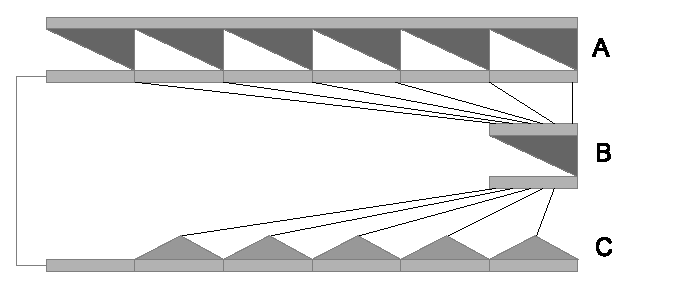
\includegraphics[width=\linewidth]{./csort/prefixsum}
\caption{Illustration of how to combine many local prefix sum computations 
 into a large one. The algorithm has three steps: A compute local prefix sums, 
 B recursively compute prefix sums on the maximums of the local prefix sum 
 calculations, C distribute summed maximums over the local results.}
\label{fig:prefixsum}
\end{figure}

\begin{figure} 
\begin{center}
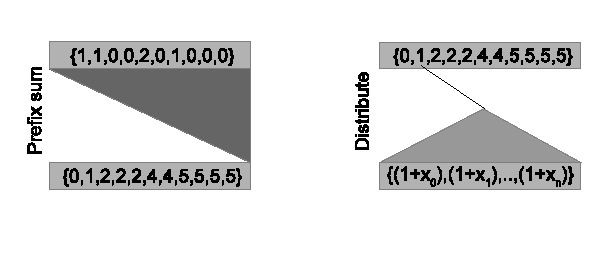
\includegraphics[width=\linewidth]{./csort/prefixzoom}
\caption{Close-up on the prefix sum and distribute operations used in Figure \ref{fig:prefixsum}.} 
%Zooms in on the shapes used in figure \ref{fig:prefixsum}. The left 
%shape symbolises a prefix sum and the right shows the distribute operation}
\label{fig:prefixzoom}
\end{center}
\end{figure}

The figure also shows what kernels we need to produce. First, something that 
performs a number of local prefix sums in parallel over the full length 
of an array is needed. The prefix sum algorithm that we implement here is 
based on divide and conquer and originates from Sklansky \cite{Sklansky}. 
% A kernel that performs the distribution (part C in the figure) is also needed. 

The code below can be thought of as a program generator. Given an integer, $n$,
it gives a prefix computation for $2^n$ elements. Here we go directly to 
generating the prefix sums operations (with the operator + hard coded) rather 
than a higher order function that can be used to more generically.

\begin{small}
\begin{Verbatim}[samepage=true]
sklansky :: Int 
            -> Pull EWord32 
            -> BProgram (Pull EWord32)
sklansky 0 arr = return arr
sklansky n arr = do 
    let arr1 = binSplit (n-1) fan arr
    arr2 <- force arr1
    sklansky (n-1) arr2
\end{Verbatim}
\end{small} 

%\begin{small}
%\begin{verbatim} 
%sklansky :: Scalar a => Int -> (Exp a -> Exp a -> Exp a)
%            -> Pull (Exp a) -> BProgram (Pull (Exp a))
%sklansky 0 op arr = return arr
%sklansky n op arr = do 
%    let arr1 = binSplit (n-1) (fan op) arr
%    arr2 <- force arr1
%    sklansky (n-1) op arr2
%\end{verbatim}
%\end{small} 

The {\tt sklansky} code above is short but still contains much that needs 
explanation. First, the type specifies that the function takes a normal 
Haskell Int and an input array ({\tt Pull EWord32}). The result is a {\tt BProgram} that 
produces a result array. 
%The code above could be thought of as a program 
%generator for a supplied number,$n$, and operation (for example (+)); it gives 
%you a program that performs all prefix sums operation on an array. 
The function {\tt binSplit} is in the Obsidian library and is used 
to implement divide and conquer algorithms. This function splits an array 
recursively a given number of times and then applies some computation on all 
parts. In this case the {\tt fan} operation implemented below is used. 

%To be able to implement prefix sum on the GPU we need to split the work 
%up into different phases. While computing a prefix sum in parallel , values 
%needs to be communicated between threads. This indicates that a kernel that 
%utilises local shared memory is a good idea. In CUDA the threads that can 
%communicate via shared memory all belong to the same block (group of threads). 
%These blocks can contain up to 1024 threads but often much fewer to 
%conserve resources and allow more blocks to run in parallel. In this example 
%a 256 threads (and elements) kernel is created. In the 
%benchmarks (section \ref{sec:Benchmarks}) prefix sum kernels of many 
%different sizes are used but all of these can be generated from the same 
%Obsidian description. In order to be able to implement a large prefix sum 
%the local kernel is also designed to output its maximal element to 
%a separate array. This separate array can be used to compute values to adjust 
%the local sums by. This follows the schema developed in \cite{LargeScan}.

%The local prefix sum is executed in parallel over the large array. 
%The large array is thus some multiple of the number of elements that the 
%local kernel can process. These sub results (both local scans and recursively 
%scaned block maximi) are then combined using another kernel called 
%{\tt distribute}. 

%\begin{verbatim} 
%sklansky :: Scalar a => Int -> (Exp a -> Exp a -> Exp a)
%            -> Pull (Exp a) -> BProgram (Pull (Exp a))
%sklansky 0 op arr = return arr
%sklansky n op arr = do 
%    let arr1 = twoK (n-1) (fan op) arr
%    arr2 <- force arr1
%    sklansky (n-1) op arr2
%\end{verbatim}

\begin{small}
\begin{Verbatim}[samepage=true]
fan arr =  a1 `conc`  fmap (+ (last a1)) a2 
    where 
      (a1,a2) = halve arr
\end{Verbatim} 
\end{small}
%\begin{small}
%\begin{verbatim} 
%fan op arr =  a1 `conc`  fmap (op c) a2 
%    where 
%      (a1,a2) = halve arr
%      c = a1 ! (fromIntegral (len a1 - 1))
%\end{verbatim} 
%\end{small}


The {\tt fan} operation splits an array down the middle and then adds 
the element at the highest index of the first half to all elements of 
the second. Then the two parts are concatenated back together. 
%The {\tt sklansky} function uses the {\tt force} function that ensures 
%that the array is computed and the elements stored in memory. This can be 
%used to introduce parallelism but also, by leaving it out, to ensure fusion 
%of computations. 

In order to obtain both the local prefix sum results and the maximum 
element of the block, a small wrapper function is created. 

\begin{small}
\begin{Verbatim}[samepage=true]
sklanskyMax :: Int 
               -> Pull EWord32 
               -> BProgram (Pull EWord32, 
                            Pull EWord32)
sklanskyMax n arr = do
  res <- sklansky n arr
  return (res,singleton (last res))
\end{Verbatim}
\end{small} 
%\begin{small}
%\begin{verbatim}
%sklanskyMax :: Scalar a => Int -> (Exp a -> Exp a -> Exp a)
%     -> Pull (Exp a) -> BProgram (Pull (Exp a), Pull (Exp a))
%sklanskyMax n op arr = do
%  res <- sklansky n op arr
%  return (res,singleton (last res))
%\end{verbatim}
%\end{small} 

All this wrapper does is compute the prefix sum followed by returning the  
result and a singleton array containing the maximum, {\tt last}, element. 

%This function is currently the 
%target of much experimentation with regards to how exactly it should 
%be implemented and what exact type it should have.
This local prefix sum is run on sub-parts of the global array. The function
{\tt mapDist} splits up the array, runs a local computation on each part using
the MPs of the GPU; when it finishes, the result of that computation is an array
that remains distributed across the local memories of the GPU MPs. 

\begin{small}
\begin{Verbatim}[samepage=true]
sklanskyG :: Int 
             -> GlobPull EWord32
             -> GProgram (GlobPush EWord32, 
                          GlobPush EWord32)
sklanskyG logbsize input =
  toGProgram (mapDist (sklanskyMax logbsize) 
                      (2^logbsize) 
                      input)
\end{Verbatim}  
\end{small}
%\begin{small}
%\begin{verbatim} 
%sklanskyG :: (Num (Exp a), Scalar a)
%             => Int
%             -> GlobPull (Exp a)
%             -> GProgram (GlobPush  (Exp a), GlobPush (Exp a))
%sklanskyG logbsize input = toGProgram $
%    mapDist (sklanskyMax logbsize (+)) (2^logbsize) input
%\end{verbatim}  
%\end{small}


In the {\tt sklanskyG} function the local prefix combinator implemented 
so far is turned into a global prefix sum computation. 
The {\tt toGProgram} function takes a function from blockId to 
a {\tt BProgram} and gives back a {\tt GProgram}, that is a program running 
on the full GPU (across many MPs). 

The CUDA code generated from {\tt sklanskyG} is shown in figure
\ref{fig:genSklansky}. Writing that type of CUDA code by hand is both
tedious and error prone. The Obsidian code is both shorter, more
compositional and easier to read.

One kernel remains to be implemented, {\tt distribute}.

\begin{small}
\begin{Verbatim}[samepage=true]
distribute :: EWord32 
              -> GlobPull EWord32
              -> GlobPull EWord32 
              -> GlobPull EWord32
distribute bs maxs inputs = zipWithG (+) maxs' inputs 
  where 
    maxs' = repeat bs maxs
    repeat n = ixMap (\ix -> ix `div` n)
\end{Verbatim} 
\end{small}
%\begin{small}
%\begin{verbatim} 
%distribute :: Num a => Exp Word32 -> GlobPull a 
%              -> GlobPull a -> GlobPull a
%distribute bs maxs inputs = zipWithG (+) maxs' inputs 
%  where 
%    maxs' = repeat bs maxs
%    repeat n gp = ixMap (\ix -> ix `div` n) gp 
%\end{verbatim} 
%\end{small}
%repeat n (GlobPull ixf) = GlobPull $ \ix -> ixf (ix `div` n) 

The {\tt distribute} kernel takes three inputs, a number, $n$,  and two global pull 
arrays. The elements of the first array are repeated $n$ times and then 
the result is element wise added to the second input array. The code generated 
from this kernel is shown in figure \ref{fig:genDistrib}. The 
{\tt distribute} kernel is used in the implementation of a large prefix sum 
(over more elements then what can fit in shared memory) from local prefix sum 
computations. This is indicated in figure~\ref{fig:prefixsum}.

\begin{figure} 
\newcommand{\myfontsize}{\fontsize{7}{9}\selectfont}
{\myfontsize
\begin{verbatim} 
__global__ void sklansky(uint32_t *input0,
                         uint32_t *output0,
                         uint32_t *output1){
  extern __shared__ unsigned char sbase[];
  ((uint32_t *)sbase)[tid] = 
    (((tid&0x1)<0x1) 
      ? input0[((bid*32)+((tid&0xFFFFFFFE)|(tid&0x1)))] 
      : (input0[((bid*32)+((tid&0xFFFFFFFE)|0x0))]+
         input0[((bid*32)+((tid&0xFFFFFFFE)|(tid&0x1)))]));
  __syncthreads();
  ((uint32_t *)(sbase + 128))[tid] = 
    (((tid&0x3)<0x2) 
      ? ((uint32_t *)sbase)[((tid&0xFFFFFFFC)|(tid&0x3))] 
      : (((uint32_t *)sbase)[((tid&0xFFFFFFFC)|0x1)]+
         ((uint32_t *)sbase)[((tid&0xFFFFFFFC)|(tid&0x3))]));
  __syncthreads();
  ((uint32_t *)sbase)[tid] = 
    (((tid&0x7)<0x4) 
      ? ((uint32_t *)(sbase+128))[((tid&0xFFFFFFF8)|(tid&0x7))] 
      : (((uint32_t *)(sbase+128))[((tid&0xFFFFFFF8)|0x3)]+
        ((uint32_t *)(sbase+128))[((tid&0xFFFFFFF8)|(tid&0x7))]));
  __syncthreads();
  ((uint32_t *)(sbase + 128))[tid] = 
    (((tid&0xF)<0x8) 
      ? ((uint32_t *)sbase)[((tid&0xFFFFFFF0)|(tid&0xF))] 
      : (((uint32_t *)sbase)[((tid&0xFFFFFFF0)|0x7)]+
         ((uint32_t *)sbase)[((tid&0xFFFFFFF0)|(tid&0xF))]));
  __syncthreads();
  ((uint32_t *)sbase)[tid] = 
    ((tid<0x10) 
      ? ((uint32_t *)(sbase+128))[tid] 
      : (((uint32_t *)(sbase+128))[0xF]+
         ((uint32_t *)(sbase+128))[tid]));
  __syncthreads();
  ((uint32_t *)(sbase + 128))[tid] = ((uint32_t *)sbase)[tid];
  if (tid<1){
    ((uint32_t *)(sbase + 256))[tid] = ((uint32_t *)sbase)[31];
  }
  __syncthreads();
  output0[((bid*32)+tid)] = ((uint32_t *)(sbase+128))[tid];
  if (tid<1){
    output1[(bid+tid)] = ((uint32_t *)(sbase+256))[tid];
  }
}
\end{verbatim} 
}
\caption{CUDA code generated from the Obsidian {\tt sklanskyG} prefix sum program. 
 This example shows the 32 element version of the prefix sum computation}
\label{fig:genSklansky} 
\end{figure}

\begin{figure} 
\begin{small}
\begin{verbatim} 
__global__ void distribute(uint32_t s0, 
                           uint32_t *input1,
                           uint32_t *input2,
                           uint32_t *output0){
  output0[((bid*bDim)+tid)] = 
      (input1[(((bid*bDim)+tid)/s0)]+
       input2[((bid*bDim)+tid)]);
  
}
\end{verbatim} 
\end{small}
\caption{CUDA code generated from the Obsidian {\tt distribute} function.}
\label{fig:genDistrib} 
\end{figure}

\subsection{A note about generated code} 

All generated code shown in this paper has been edited slightly by hand. This 
is partly to increase readability but also to conserve space. The changes 
that have been made are entirely cosmetic. Line breaks have been inserted in too
long lines. All occurrences of {\tt blockIdx.x}, {\tt blockDim.x} and 
{\tt threadIdx.x} have been replaced with {\tt bid}, {\tt bDim} and {\tt tid}.
Some decimal constants have been changed to hexadecimal.
No other changes have been made. 


%\FloatBarrier
 

% insert better head of section here 
\section{Implementing counting sort in Obsidian} 
\label{sec:parallel}

%This section shows the implementations of the various kernels 
%involved in our two variants of counting sort. The prefix sum 
%computation that is used does not vary in the implementations and 
%is shown in section \ref{sec:sklansky}. 

%Two different kinds 
%of {\em histogram} and {\em reconstruct} kernels are developed. 
%The kernels involved in implementing the prefix sum used between the 
%histogram and reconstruct phases are shown in section \ref{sec:Obsidian}.

%This section outlines the implementation of the different kernels 
%required by the counting sort algorithm. The main parts are 
%computing the {\em histogram}, {\em prefix sums} and the {\em reconstruct} 
%phase. 

%The prefix sums computation consists of 2 different kernels while the 
%two other phases are performed by a single kernel. The prefix sums are computed
%in parallel following a scheme originally designed by 
%J. Sklansky \cite{Sklansky}.  

%Initially, we assumed that in order to tweak the performance of this algorithm 
%we would substitute various prefix sums networks in the place of the Sklansky 
%network and evaluate the performance difference. It may still be the case 
%that the parallel prefix network used is an important aspect in the 
%performance of this algorithm. But for many data sets the execution time 
%of the reconstruct kernel completely dominates. In this paper we use two 
%different versions of the same Sklansky network. One implemented using pull 
%arrays and the other utilising push arrays. 

%is it J. Sklansky? (whats the J for ?) 
%Lots of the above should move to discussion, right ? 

%\subsection{Counting sort}

%The missing kernels in order to implement counting sort is histogram,
%which counts occurrences of values in the input, and reconstruct, which
%outputs the final sorted array.

\subsection{Histogram} 

When computing the histogram, atomic operations are needed. Index $i$
in the histogram array is incremented for each occurrence of the value
$i$ in the input array, and if there are multiple occurrences of $i$
then multiple threads will try to increment, leading to a possible race.
CUDA atomic operations must be applied to data stored at an actual memory 
location. This does not fit very well into our setting with virtual arrays 
(arrays that do not necessarily represent data in memory). But in Obsidian 
it is possible to drop down to a low enough level of abstraction to still 
implement this function. However, we are searching for suitable higher level 
abstractions to apply here.

%\begin{small}
%\begin{Verbatim}[samepage=true] 
%histogram :: GlobPull (EInt32) -> Final (GProgram (GlobPull (EWord32)))
%histogram (GlobPull ixf) = Final $
%      do global <- Output $ Pointer (typeOf (undefined :: EWord32))
%         forAllT $ \gix ->
%           do AtomicOp global (int32ToWord32 (ixf gix))  AtomicInc
%              return ()
%         return (GlobPull (\i -> index global i))
%\end{Verbatim}
%\end{small}

\begin{small} 
\begin{Verbatim}[samepage=true] 
histogram :: GlobPull EInt32 
             -> GProgram ()
histogram gpull = do
  global <- Output $ Pointer Word32 
  forAllT $ \gix -> 
     atomicOp global 
              (int32ToWord32 (gpull ! gix)) 
              AtomicInc
\end{Verbatim} 
\end{small} 

Below, the code generated from this Obsidian program is shown.

\begin{small}
\begin{Verbatim}[samepage=true] 
__global__ void histogram(int32_t *input0,
                          uint32_t *output0){
  
  atomicInc(output0+(uint32_t)(input0[((bid*bDim)+tid)]),
            0xFFFFFFFF);
  
}
\end{Verbatim}
\end{small}


The generated code uses \verb!atomicInc! to increment a value in an
array. The function is conditional, incrementing only if the value in
memory is larger than the second argument. Since we always want to
increment, no matter the value in memory, we've supplied {\tt
  0xFFFFFFFF}, which is the largest possible value.

The Obsidian code and the CUDA code are very similar in size and complexity. 
However, an important advantage of the Obsidian code is that it composes better
than the CUDA code. If the input to {\tt histogram} was a {\tt
  GlobPull} array produced by some other Obsidian function, then the
two functions would be fused, typically generating much faster code
and not allocating memory for the fused array.

%\newpage
\subsection{Reconstruct}

The kernel for the reconstruct step uses one thread per element in the
input array. Each thread is implemented as a loop to write its
corresponding element as many times as it should occur in the output.

\begin{small}
\begin{Verbatim}[samepage=true] 
reconstruct :: GlobPull EWord32 
               -> GlobPush EInt32
reconstruct (GlobPull ixf) = GlobPush f
  where f k = 
    do forAllT $ \gix ->
         let startIx = ixf gix 
         in  SeqFor (ixf (gix + 1) - startIx) $ \ix ->
               k (word32ToInt32 gix) (ix + startIx)
\end{Verbatim}
\end{small}

The generated CUDA code for \verb!reconstruct! can be seen
below. Modulo syntax and some index manipulation, the code is very
similar to the Obsidian code.

\begin{small}
\begin{Verbatim}[samepage=true]
__global__ void reconstruct(uint32_t *input0,
                            int32_t *output0){
  
  for (int i1 =  0;
       i1 < (input0[(((bid*bDim)+tid)+1)]-
             input0[((bid*bDim)+tid)]);
       i1++)
  {
    output0[(i1+input0[((bid*bDim)+tid)])] = 
      (int32_t)(((bid*bDim)+tid));
    
  }
  
}
\end{Verbatim}
\end{small}

Again, the difference between Obsidian and CUDA might seem small, but
just as above, the code in Obsidian composes better.

\section{Implementing occurrence sort in Obsidian} 
\label{sec:occur}

Occurrence sort uses an {\tt occurs} kernel instead of a 
histogram. The result of the occurs computation is an array with a one 
at indices corresponding to values occurring in the input array. The 
reconstruction of the sorted (and duplicate free) array is also done 
slightly differently.

\subsection{Occurs}

The occurs kernel is implemented by using the {\tt scatterGlobal} 
function from the Obsidian library. This function takes two arrays, one of 
indices to write to and a second of elements to write. In this case, it 
is applied to the input array and an array containing all ones 
({\tt replicateG 1}). 

\begin{small}
\begin{Verbatim}[samepage=true] 
occurs :: GlobPull EInt32 -> GlobPush EWord32
occurs elems = 
  scatterGlobal (fmap int32ToWord32 elems) (replicateG 1)
\end{Verbatim}
\end{small} 

The CUDA code generated from this function is shown below. 

\begin{small}
\begin{Verbatim}[samepage=true] 
__global__ void occurs(int32_t *input0,
                       uint32_t *output0){
   
  output0[(uint32_t)(input0[((bid*bDim)+tid)])] = 1;
  
}
\end{Verbatim} 
\end{small} 

When running this code, it is possible that many threads write to the same 
target element. Since all are writing a one, no atomic operations are needed; 
the result will still be one. 

It is worth comparing the Obsidian code for the {\tt histogram} kernel
and the {\tt occurs} kernel. The {\tt histogram} kernel is highly
imperative in nature, and requires atomic operations to manage
synchronisation between threads. The {\tt occurs} kernel, on the other
hand, has a very straightforward data-parallel implementation. Not only
is it simpler, but as we will see in section \ref{sec:Benchmarks}, it
is also significantly faster.

\subsection{Reconstruct} 

The reconstruct kernel for the occurrence sort algorithm  is
almost identical to the kernel used for standard counting sort. The
only difference is that a conditional can be used instead of a loop. 
This can be seen as a slight optimisation; the previous version of reconstruct 
could still be used in its place. 

\begin{small}
\begin{Verbatim}[samepage=true]
reconstruct :: GlobPull EWord32 
               -> GlobPush EInt32
reconstruct (GlobPull ixf) = GlobPush f
  where f k = 
    do forAllT $ \gix ->
         let startIx = ixf gix 
         in  Cond ((ixf (gix + 1) - startIx) ==* 1) $
               k (word32ToInt32 gix) startIx
\end{Verbatim}
\end{small}

This variant of reconstruct results in the generated code below. 

\begin{small}
\begin{Verbatim}[samepage=true]
__global__ void reconstruct(uint32_t *input0,
                            int32_t *output0){
   
  if ((input0[(((bid*bDim)+tid)+1)]-
       input0[((bid*bDim)+tid)])==1){

  output0[input0[((bid*bDim)+tid)]] = 
      (int32_t)(((bid*bDim)+tid));
  
  }

}
\end{Verbatim}
\end{small}





%\subsection{Histogram computations} 
%
%There are two different variants of the histogram computation used 
%in our counting sort implementations. The first does not really create 
%a histogram but creates an array that indicates what elements occurred. A
%one in position $p$ indicates that $p$ was present in the input array. 
%
%There is also a full histogram used in the full version of counting sort. 
%Here if $n$ occurs at position $p$ in the result array it indicates that 
%$p$ occurs $n$ times in the input array. 

%\subsubsection{First histogram} 
%
%First we implement the histogram for the counting sort variant that removes
%duplicate elements. This function is not really a histogram, but rather 
%it places a one at each index that correspond to an element in the data array.
%The first histogram is implemented by using the {\tt scatterGlobal} 
%function from the Obsidian library. This function takes two arrays, one of 
%indices to write to and a second of elements to write. In this case it 
%is applied to the input array and an array containing all ones 
%({\tt replicateG 1}). 
%
%\begin{small}
%\begin{Verbatim}[samepage=true] 
%histogram :: GlobPull (EInt32) -> GlobPush (EWord32)
%histogram elems = 
%  scatterGlobal (fmap int32ToWord32 elems) (replicateG 1)
%\end{Verbatim}
%\end{small} 
%
%The CUDA code generated from this function is shown below. 
%
%\begin{small}
%\begin{Verbatim}[samepage=true] 
%__global__ void histogram(int32_t *input0,uint32_t *output0){
%   
%  output0[(uint32_t)(input0[((bid*bDim)+tid)])] = 1;
%  
%}
%\end{Verbatim} 
%\end{small} 
%
%When running this code it is possible that many threads write to the same 
%target element. Since all are writing a one no atomic operations are needed, 
%the result will still be one. 

%\subsubsection{Full histogram}
%
%When implementing the full histogram atomic operations are needed. In this 
%variant index $i$ in the histogram array is incremented for each occurrence 
%of the value $i$ in the input array. 
%CUDA atomic operations must be applied to data stored at an actual memory 
%location. This does not fit very well into our setting with virtual arrays 
%(arrays that do not necessarily represent data in memory). But in Obsidian 
%it is possible to drop down to low enough level of abstraction to still 
%implement this function. However, we are searching for suitable higher level 
%abstractions to apply here. 

%\begin{small}
%\begin{Verbatim}[samepage=true] 
%fullHistogram :: GlobPull (EInt32) -> Final (GProgram (GlobPull (EWord32)))
%fullHistogram (GlobPull ixf) = Final $
%      do global <- Output $ Pointer (typeOf (undefined :: EWord32))
%         forAllT $ \gix ->
%           do AtomicOp global (int32ToWord32 (ixf gix))  AtomicInc
%              return ()
%         return (GlobPull (\i -> index global i))
%\end{Verbatim}
%\end{small}
%
%\begin{small}
%\begin{Verbatim}[samepage=true] 
%__global__ void fullHistogram(int32_t *input0,uint32_t *output0){
%  
%  atomicInc(output0+(uint32_t)(input0[((bid*bDim)+tid)]),0xFFFFFFFF);
%  
%}
%\end{Verbatim}
%\end{small}
%
%
%The generated code uses atomicInc to increment a value in an array. 
%The second argument {\tt 0xFFFFFFFF} is a maximum required by CUDAs atomicInc, 
%the value is incremented if it is less than this value. To implement a count, 
%the maximum possible value is used as this argument. 


%\subsection{Array reconstruction} 
%
%After the histogram computation and the prefix sum that computes the array 
%we call the position arrays is done its time to reconstruct the sorted output. 
%
%\subsubsection{Reconstruct} 
%
%The first variant of reconstruct is for the duplicate removing counting sort. 
%It takes the original data array and the position array as input. If element 
%$i$ is in the data array it is written to the position that is pointed out
%by index $i$ in the position array. 
%
%\begin{small} 
%\begin{Verbatim}[samepage=true] 
%reconstruct :: GlobPull (EInt32) -> GlobPull (EWord32)
%               -> GlobPush (EInt32)
%reconstruct inp pos = scatterGlobal (ixMap f pos) inp  
%  where
%    f gix = fmap int32ToWord32 inp ! gix
%\end{Verbatim}
%\end{small} 
%
%
%\begin{small}
%\begin{Verbatim}[samepage=true] 
%__global__ void kernel(int32_t *input0,uint32_t *input1,int32_t *output0){
%   
%  output0[input1[(uint32_t)(input0[((bid*bDim)+tid)])]] = 
%   input0[((bid*bDim)+tid)];
%  
%}
%\end{Verbatim}
%\end{small}
%
%There is a way to implement an optimised version of reconstruct for 
%the counting sort that removes duplicates. This version does not take the 
%original data array as input. Instead the output data is recreated from the 
%position array alone.  
%
%\begin{small}
%\begin{Verbatim}[samepage=true]
%reconstruct' :: GlobPull (Exp Word32) -> GlobPush (Exp Int32)
%reconstruct' (GlobPull ixf) = GlobPush f
%  where f k = do forAllT $ \gix ->
%                   let startIx = ixf gix in
%                   Cond ((ixf (gix + 1) - startIx) ==* 1) $
%                      k (word32ToInt32 gix) startIx
%\end{Verbatim}
%\end{small}
%
%\begin{small}
%\begin{Verbatim}[samepage=true]
%__global__ void reconstruct_opt(uint32_t *input0,int32_t *output0){
%   
%  if ((input0[(((bid*bDim)+tid)+1)]-input0[((bid*bDim)+tid)])==1){
%
%  output0[input0[((bid*bDim)+tid)]] = (int32_t)(((bid*bDim)+tid));
%  
%  }
%
%}
%\end{Verbatim}
%\end{small}




%\begin{small}
%\begin{Verbatim}[samepage=true] 
%
%reconstruct :: Exp Word32 
%            -> GlobalArray Pull (Exp Word32) 
%            -> GlobalArray Pull (Exp Word32) 
%            -> Kernel (GlobalArray Push (Exp Word32))
%reconstruct l inp pos = return $ 
%  flip mkGlobalPushArray l $ \k ->
%    forAllGlobal (globLen inp) $ \i ->
%      k (pos ! (inp ! i),inp ! i)
%
%\end{Verbatim} 
%\end{small}


%\subsubsection{Full reconstruction} 

%\begin{small}
%\begin{Verbatim}[samepage=true] 
%fullReconstruct :: GlobPull (EWord32) -> GlobPush (EInt32)
%fullReconstruct (GlobPull ixf) = GlobPush f
%  where f k = do forAllT $ \gix ->
%                   let startIx = ixf gix in
%                   SeqFor (ixf (gix + 1) - startIx) $ \ix ->
%                      k (word32ToInt32 gix) (ix + startIx)
%\end{Verbatim}
%\end{small}
%
%\begin{small}
%\begin{Verbatim}[samepage=true]
%__global__ void kernel(uint32_t *input0,int32_t *output0){
%  
%  for (int i1 =  0;
%       i1 < (input0[(((bid*bDim)+tid)+1)]-input0[((bid*bDim)+tid)]);
%       i1++)
%  {
%    output0[(i1+input0[((bid*bDim)+tid)])] = (int32_t)(((bid*bDim)+tid));
%    
%  }
%  
%}
%\end{Verbatim}
%\end{small}



%\subsection{The CUDA framework MOVE TO BENCHMARK SECTION} 

%Given the generated code for all the kernels described previously it is now 
%possible to construct the complete algorithm in CUDA by simply providing the 
%skeleton that launches them. This involves allocation memory on the CUDA device 
%for all intermediate results (here intermediate means between the launches of two 
%kernels). Data needs to be copied to the device and then the kernels launched.
%for example, the kernel generated from the Obsidian histogram function can 
%be launched on the GPU by issuing: 

%\begin{small}
%\begin{Verbatim}[samepage=true] 
%histogram<<<nblocks, nthreads,0>>>(dvalues,0,histresult);
%\end{Verbatim} 
%\end{small}

%This indicates that {\tt histogram} should be started using {\tt nblocks}
%number of blocks of each {\tt nthreads} number of threads and no shared 
%memory. 
%In the current status of Obsidian this ``kernel coordination'' code needs 
%to be described in CUDA. 

%Definitely not room for the actual code here! (Maybe not even pseudocode) 


 
%The histogram kernel is operating on a large global input array. It looks 
%at each element in the input array and then puts a one in the output 
%array to signal the presence of a particular value. 

%This particular kernel does not need to use any local memory on the GPU and 
%there is no communication between threads. To implement this kernel it is 
%suitable to use Obsidian's global arrays.
 

%The kernel takes two inputs, a maximum length related to the size of the largest 
%element in the input data and a global array containing that data. A global 
%push array is created that contains a one at each index which corresponds to a
%value in the input data.

% \subsection{Computing prefix sums} 

%The prefix sum computation is different from the histogram one. Here threads
%needs to communicate and thus a kernel that utilises the GPU shared memory 
%is more suitable. 

%\begin{small}
%\begin{Verbatim}[samepage=true] 
%sklansky :: (Choice a, Syncable (Array Pull) a) 
%         =>Int
%         -> (a -> a -> a)
%         -> Array Pull a
%         -> Kernel (Array Pull a)
%sklansky 0 op = pure id
%sklansky n op = pure (twoK (n-1) (fan op)) 
%              ->- sync 
%              ->- sklansky (n-1) op 
%
%fan op arr = conc (a1, fmap (op c) a2) 
%    where 
%      (a1,a2) = halve arr
%      c = a1 ! (fromIntegral (len a1 - 1)) 
%\end{Verbatim} 
%\end{small}
%
%With this Obsidian code CUDA kernels can be generated that operate on certain 
%small sized sub arrays (called blocks). The factors that limit the number of 
%elements that the kernel can operate upon are size of shared memory and number 
%of threads per block that the CUDA device can launch. For this particular 
%kernel the number of threads limits it to operate on a maximum of 512 or 
%1024 elements depending on generation of GPU.  
%In order to build a large parallel prefix from these small ones an approach 
%similar to the one taken in \cite{LargeScan} is implemented. This requires 
%that the {\tt sklansky} kernel also outputs the maximum element from each 
%small block into a separate array of ``block maximums''. On the 
%block maximums a second prefix sum is computed and the result of that is then 
%distributed over the elements of the other blocks in the appropriate way. 
%So, to implement this the {\tt sklansky} function is modified into a function 
%that also outputs the block-maxima to a separate array: 
%
%\begin{small} 
%\begin{Verbatim}[samepage=true] 
%sklanskyM n op = sklansky n op ->- pure pairMax 
%  where
%    pairMax a = (a,
%                 let i = fromIntegral (len a - 1)
%                 in singleton (a ! i))

%\end{Verbatim}
%\end{small}

%The next step is the kernel that distributes (scanned) block-maximums. This is 
%again a kernel that does not need to use any local storage or communication
%between threads so the global array approach is suitable. The  inputs 
%to this kernel is, the block size, the array block maximums and the array 
%of elements we operate on. The output is an array where the element i of 
%the block maximums array is combined with each element in block i+1 of the 
%input data array.  

%\begin{small}
%\begin{Verbatim}[samepage=true] 
%distribute :: Exp Word32 
%           -> (GlobalArray Pull (Exp Word32), 
%               GlobalArray Pull (Exp Word32)) 
%           -> Kernel (GlobalArray Push (Exp Word32)) 
%distribute bsize (bmaxs,arr) = pure distr arr1
%    where 
%      distr arr = 
%          pushGlobal (zipWithGlobal (+) 
%                                    (expand bsize bmaxs) 
%                                    arr)
%      expand n arr =
%        mkGlobalPullArray (\ix -> arr ! (ix `div` n))  
%                          (globLen arr * n) 
%\end{Verbatim} 
%\end{small}

%Distribute works by expanding the array of block maximums, that is repeating each 
%of its elements a certain number of times and then performing a traditional 
%{\tt zipWith} operation with the values array. 

%The Obsidian code for {\tt sklansky} uses the {\tt conc} operation and the 
%generated code has an unfortunate conditional that is executed by each thread.
%Because of this another version was implemented using push arrays. The push 
%array version uses half as many threads and each thread computes both 
%branches of the conditional from the previous version. 

%\begin{small}
%\begin{Verbatim}[samepage=true] 
%ilv2v :: Choice a => Int -> (a -> a -> a) -> 
%                    Array Pull a -> Array Push a
%ilv2v i g arr 
%   = mkPushArray (\k -> a5 !* k *>* a6 !* k) n
%  where
%    n  = len arr
%    n2 = n `div` 2
%    a1 = resize (ixMap left arr) (n-n2) 
%    a2 = resize (ixMap right arr) (n2)  
%    a3 = resize (ixMap mid arr) (n2) 
%    a4 = zipWith g a3 a2
%    a5 = ixMap left (push a1)
%    a6 = ixMap right (push a4)
%    left = insertZero i
%    right = flipBit i  . left
%    mid = (.|. oneBits i) . left
%
%fan1 n op arr = ilv2v n op arr
%  
%%sklansky1 n op = [ilv2v i op | i <- [0..(n-1)]]
%\end{Verbatim} 
%\end{small}
%assumes we provide compose.
%maybe we should assume ilv2v is a library function 
%  and just explain what it does. 
%maybe Mary wants to tweak the above slightly ? 

%For space reasons we omit all examples of generated code. For many examples 
%of the kind of code Obsidian generates see references \cite{JSLIC,PUSH}. 


\subsection{Performance evaluation} 
\label{sec:Benchmarks}

\FloatBarrier

This section presents the experimental results. Our implementations of
counting sort are compared to the implementation of sorting from the
Thrust library \cite{THRUST}. Thrust is a C++ library, developed by
NVIDIA, which provides abstractions similar to the standard template
library, but targets the GPU. The reason we have chosen to compare with
Thrust is that it has similar goals to Obsidian: to provide high-level 
constructs while generating efficient GPU code.

All the data being sorted in the measurements are 32 bit unsigned
integer valued keys.
The convention used in the charts is that the y-axis represents time in ms. 
The different experiments are called {\em sorted} for sorting of an 
already sorted array, and {\em unique} for sorting of randomised arrays where each 
element occurs exactly once. There are also a number of experiments called 
T$x$ for a number $x$;  the arrays used in these experiments contain
elements from an interval of numbers (0 to $2^x-1$). 

Figures \ref{fig:chart1} and \ref{fig:chart3} show the results of
comparing our full counting sort to Thrust sort and occurrence sort
 to Thrust's {\tt sort} and {\tt unique} functions.
%% Figure \ref{fig:chart1}  show the results of
%% comparing our full counting sort to Thrust sort and our duplicate
%% removing sort to Thrust sort followed by unique.
Our implementation of
counting sort consistently outperforms Thrust, except for small ranges
of values. The reason counting sort performance degrades is that the
number of threads used in the reconstruct step is proportional to the
range, and therefore at small ranges the execution becomes more
sequential.

We compare occurrence sort to sort followed by unique from
the Thrust library because that seems to be the current best practice
\cite{REMOVEDUPS}. Our implementation is always at least twice as fast
but in many cases it outperforms Thrust by more than a factor of four.
Our method is clearly beneficial for removing duplicates.

%We are comparing 
%our implementations of counting sort to the sorting algorithm present 
%in the Thrust library. 
%The counting sort that removes duplicates is compared to Thrust's sort 
%followed by unique (unique removes all but one element in groups 
%of consecutively equal elements). These results can be found in 
%figures \ref{fig:chart1} and \ref{fig:chart3}. 

%We also compare our two variants of counting sort directly to each
We also compare occurrence sort and counting sort to each 
other.  The result of this is shown in figure \ref{fig:chart2}. We
can see that the occurrence sort is typically a factor of
two faster than the regular sorting algorithm. The speedup comes from
the fact that the {\tt occurs} kernel doesn't need to perform any kind
of synchronisation, whereas the {\tt histogram} kernel needs to use
atomic operations.

The charts included in this paper show the performance when sorting eight
respectively 32 million ($2^{23}$ resp. $2^{25}$) elements. However, we 
ran all benchmarks with a number of elements, $N$, equal to $2^{n}$ for $n$ 
between 20 and 25. We found that the interesting comparison is not in what 
happens as $N$ grows larger but rather what happens as we vary the ranges 
of the elements contained in the arrays. 
%% when the ranges of the 
%% elements contained in the array is increased. 

All timing was performed on a system with an NVIDIA GTX670 GPU.  
 
\begin{figure*}
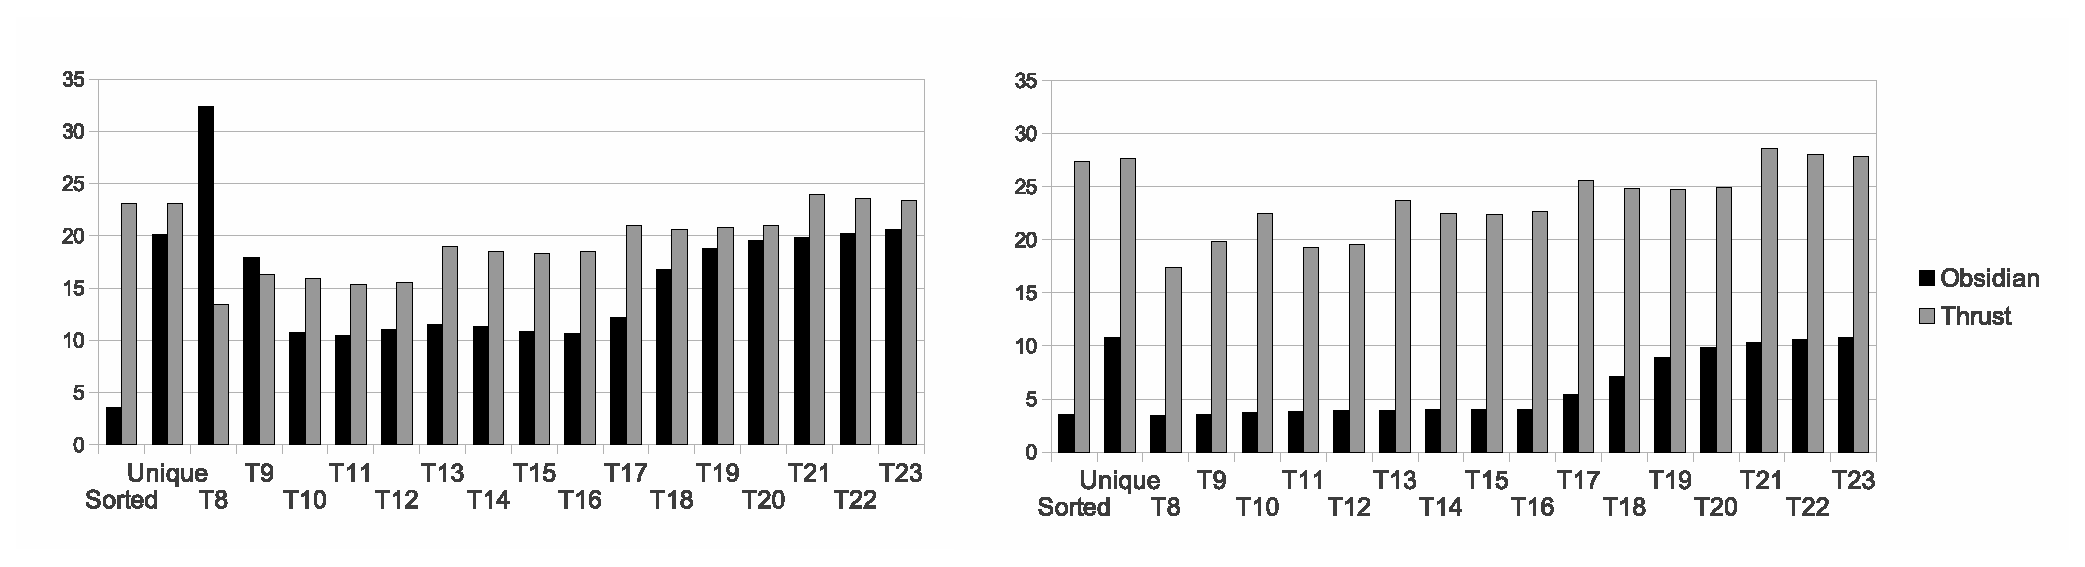
\includegraphics[width=\linewidth]{./csort/chart1}
\caption{On the left, counting sort is compared to the Thrust library. 
On the right, occurrence sort is compared to the {\tt sort} followed by {\tt unique} 
function in Thrust. Both charts show running time for 8 Million elements.}
%The left chart shows running time of full counting sort compared to 
%the sort function in the Thrust library. The right chart shows running time 
%of counting sort that removes duplicates compared to the sort followed by 
%unique function of the Thrust library. 8 Million elements where used in these 
%experiments.}
\label{fig:chart1}
\end{figure*}

\begin{figure*}
\includegraphics[width=\linewidth]{./csort/chart3}
\caption{This chart shows same comparison as figure \ref{fig:chart1}, but for 
32 Million elements.}
%The left chart shows running time of full counting sort compared to 
%the sort function in the Thrust library. The right chart shows running time 
%of counting sort that removes duplicates compared to the sort followed by 
%unique function of the Thrust library. 32 Million elements where used in 
%these experiments.}
\label{fig:chart3}
\end{figure*}


\begin{figure*}
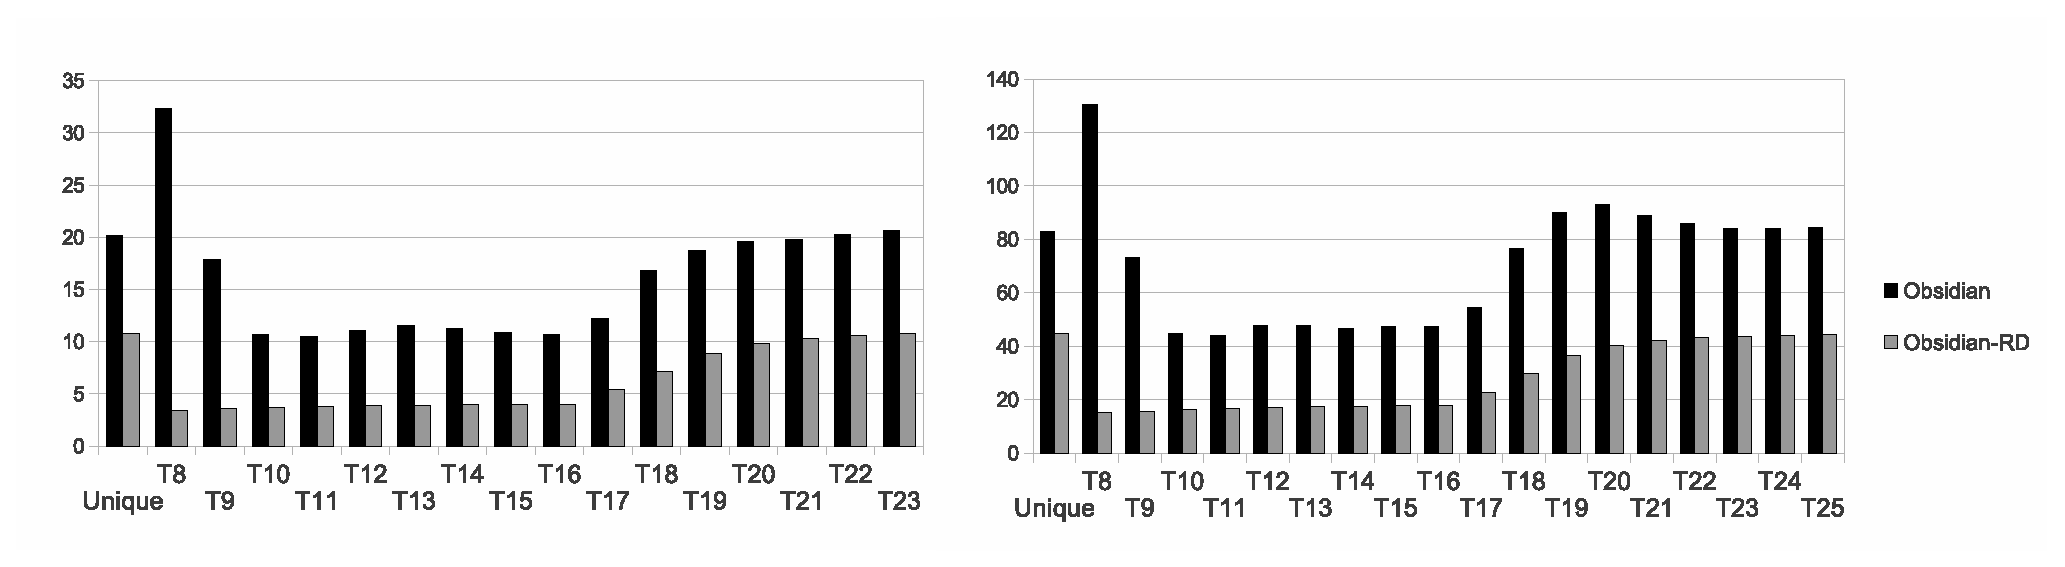
\includegraphics[width=\linewidth]{./csort/chart2}
\caption{These two charts compares occurrence sort to  counting sort. 
The left chart is for 8 Million elements and the right chart is 
for 32 Million elements.}
\label{fig:chart2}
\end{figure*}



\subsubsection{CUDA framework for the benchmarks}


To obtain the timing measurements above, a 
framework\footnote{Source code needed to repeat our experiments is available at \url{www.cse.chalmers.se/~joels/csort.html}} 
written in CUDA was used. 
This framework looks very similar to the CUDA code in figure \ref{fig:cudaCoord}. 
The main difference is that a number of kernels are run in sequence, as 
shown in figure \ref{fig:csortframe}. The timing is performed on the GPU 
computation only, as illustrated by figure \ref{fig:timing}.

\begin{figure} 
\begin{small}
\begin{verbatim} 
float total_time;

cudaEventRecord(start,0);
for (int i = 0; i < 1000; ++i) { 
    // perform counting sort. 
}
cudaEventRecord(stop,0);
cudaEventSynchronize(stop);
   
cudaEventElapsedTime(&total_time,start,stop);
\end{verbatim}
\end{small}
\caption{The timing methodology used in performance experiments. A CUDA event 
is recorded before and after the execution on the GPU. Their respective recorded times
are then compared.}
\label{fig:timing}
\end{figure}



\begin{figure} 
\begin{small}
\begin{verbatim} 
histogram<<<NB,BS,0>>>(dinput,dhistoutput);
  
scan256<<<NB,BS,2052>>>
    (dhistoutput,dscanoutput+1,dmaxs+1);
  
//dmaxs needs to be scaned (dmaxs2 is ignored) 
scan256<<<SMALL,BS,2052>>>
    (dmaxs+1,dmaxs+1,dmaxs1+1); 

scan16<<<1,SMALL,132>>>
    (dmaxs1+1,dmaxs1+1,dmaxs2); 

// distribute can be in-place regarding dresult 
// since it reads and writes in the exact 
// same location (per thread)
distribute<<<SMALL,BS,0>>>
    (BS,dmaxs1,dmaxs+1,dmaxs+1);
distribute<<<NB,BS,0>>>
    (BS,dmaxs,dscanoutput+1,dscanoutput+1);

reconstruct<<<NB,BS,0>>>
    (dscanoutput,dresult);   
\end{verbatim}
\end{small}
\caption{The kernel launch sequence used in the timing of counting sort for 
1 Million elements. Any other input data size would vary only some of the prefix 
sum (scan in the code) sizes.}
\label{fig:csortframe}
\end{figure}

% \FloatBarrier

%\begin{figure}
%\includegraphics[width=\linewidth]{./img/chartObs2M}
%\caption{Another chart example!}
%\label{fig:chart2}
%\end{figure}

%\begin{figure}
%\includegraphics[width=\linewidth]{./img/chartObs4M}
%\caption{Another chart example!}
%\label{fig:chart2}
%\end{figure}

%\begin{figure}
%\includegraphics[width=\linewidth]{./img/chartObs8M}
%\caption{Another chart example!}
%\label{fig:chart2}
%\end{figure}


%\begin{figure}[ht]
%\begin{minipage}[b]{0.5\linewidth}
%\centering
%\includegraphics[width=\textwidth]{./img/chartObs4M}
%\caption{This is to the left}
%\label{fig:figure1}
%\end{minipage}
%\hspace{0.5cm}
%\begin{minipage}[b]{0.5\linewidth}
%\centering
%\includegraphics[width=\textwidth]{./img/chartObs8M}
%\caption{This is to the right}
%\label{fig:figure2}
%\end{minipage}
%\end{figure}

%\begin{figure}
%\includegraphics[width=\linewidth]{./img/chart3}
%\caption{Shows execution of the counting sort algorithm on 4 million 
%         random elements.}
%\label{fig:chart3}
%\end{figure}

%Figures \ref{fig:chart1},\ref{fig:chart2} and \ref{fig:chart3} show how our algorithm 
%compares to a thrust implementation for 4,8 and 16 million elements in 
%various ranges.
 
% >>> What can be said more about the numbers ???


\section {Discussion}

%% ** TODO. Mention CSE. warp-related opt.

Push arrays form a new approach to array representation in DSELs.
We do not know of similar approaches in the literature, despite
the fact that the notions of demand and data flow
may feel familiar to the reader who considers Pull and Push arrays.
The addition of Push arrays to Obsidian seems highly beneficial. With 
this new feature, the user gains finer grained control over the code generated
and the resulting CUDA kernels perform considerably better than before.
This 
was illustrated in the series of sorters explored in section~\ref{sec:MARY}.
The performance of {\tt vsort} is sufficiently good that it
can be used as a first phase in a larger sorter (written in CUDA) that
can sort 16M elements in 96 ms, while an i7-920 CPU takes
around 2740 ms. Further speed improvements look possible, both in the coordination code
and in the kernels. An obvious next step would be to investigate the generation of the {\tt iSwap} and
{\tt vSwap} kernels from Obsidian. (This is not currently possible because of assumptions that we made about the interfaces to kernels and about how {\em thread ids} are used. We will look into ways to relax
our assumptions.)

The series of kernels also illustrates how the use of combinators brings a form of reuse, and makes design exploration easier. Our experience of using similar combinators in the Lava hardware
description language~\cite{LavaSorter} was that a relatively small set of combinators went a long way. So, although we introduced three
combinators here, {\tt ilv}, {\tt vee} and {\tt ilvVee}, which
includes the other two, we do not believe that every new kernel development exercise would demand a completely new set of combinators.
We expect to provide the user with a well-documented set of combinators,
so that users can get access to this style of programming without having
to develop their own combinators, and without having to think too much
about bit-hacking.
The bit-manipulation approach chosen to define our combinators automatically
created functions that apply to sub-sequences of the input that
are of an appropriate length.

In this paper, we made combinators for the special case of two input, two
output operations (built from two two-input funtions that we typically called
{\tt f} and {\tt g}). 
This approach should be generalised to deal with blocks that have $2^k$ inputs
and outputs.
Also, we made a compound combinator from {\tt ilv} and {\tt vee},
but generalising to more than two input components would allow
for composing combinators, and indeed for recursive descriptions
that could be unrolled. Then, ignoring {\tt syncs}, a recursive description of
{\tt vsort} could be something like 
\begin{codesize}
\begin{verbatim}
vsortR 0 = id
vsortR n = bpmergeR n . ilv2 1 (vsortR (n-1))
\end{verbatim}
\end{codesize}
\noindent
It would then be necessary to optimise the code generated from
multiple applications of {\tt ilv2 1}, for example, whereas here
we have forced the user to figure out both the unrolling and the combinations.
Moving to more general combinators would also give the opportunity to
provide predefined combinators that capture more of the commonly used threading patterns (for instance $k$ indices per thread rather than the $1$ and $2$ shown here).

The integration of Push arrays into Obsidian raises some new questions.
Previously, there was a direct correspondence between the length 
of an array and the number of threads used to compute it, which
allowed the user to write an initial program without worrying about
threads at all, and then to tweak the Obsidian program if he was not satisfied
with the threading behaviour of the resulting kernel. 
Now, as can be seen in the {\tt catArrayPs} example and in the sorters, this correspondence
can be broken using Push arrays. The {\tt catArrayPs} example and two
of the sorters use half as many threads as the 
number of elements. For users who are very concerned about the speed of
the generated kernels, getting this control through using Push arrays in
a particular pattern is clearly a good thing. But adding a second, different
way to control thread use in the generated code certainly complicates matters, and further case studies are needed to confirm that the complication pays off.

The addition of Push arrays also adds the possibility to include potentially 
unsafe operations in Obsidian, for example by writing multiple array elements to the same index, or by discarding elements.
This new expressiveness will have to be carefully controlled. On the positive side, it offers the possibility to encode functions like {\tt filter} from Haskell
that
are simply not expressible using only Pull arrays. Being able to implement {\tt filter} would make programming kernels in obsidian feel much more like programming in Haskell -- a welcome loosening of the strait-jacket.
Once that is done, it will be time to develop a very simple coordination language to allow programming of entire GPU applications that make use of
the kind of small kernel building blocks developed here.





%\appendix
%\section{Appendix Title}

%This is the text of the appendix, if you need one.

\subsection*{Acknowledgments} %\acks
This research has been funded by the Swedish Foundation for
Strategic Research (which funds the Resource Aware Functional 
Programming (RAW FP) Project) and by the Swedish Research Council.


\bibliographystylecsort{alpha}
\bibliographycsort{thesis}

%\begin{thebibliography}{18}
%\providecommand{\natexlab}[1]{#1}
%% \providecommand{\url}[1]{\texttt{#1}}
%% \expandafter\ifx\csname urlstyle\endcsname\relax
%%   \providecommand{\doi}[1]{doi: #1}\else
%%   \providecommand{\doi}{doi: \begingroup \urlstyle{rm}\Url}\fi

%% \bibitem[wik()]{wikipedia}
%% Wikipedia article: Counting sort.
%% \newblock \url{http://en.wikipedia.org/wiki/Counting_sort}.

%% \bibitem[Chakravarty et~al.(2011)Chakravarty, Keller, Lee, McDonell, and
%%   Grover]{Acc}
%% M.~M. Chakravarty, G.~Keller, S.~Lee, T.~L. McDonell, and V.~Grover.
%% \newblock {Accelerating Haskell array codes with multicore GPUs}.
%% \newblock In \emph{Proc. of the sixth workshop on Declarative aspects of
%%   multicore programming}, DAMP '11. ACM, 2011.

%% \bibitem[Claessen et~al.(2012)Claessen, Sheeran, and Svensson]{PUSH}
%% K.~Claessen, M.~Sheeran, and B.~J. Svensson.
%% \newblock {E}xpressive {A}rray {C}onstructs in an {E}mbedded {GPU} {K}ernel
%%   {P}rogramming {L}anguage.
%% \newblock In \emph{Proceedings of the 7th workshop on Declarative aspects and
%%   applications of multicore programming}, DAMP '12, 2012.

%% \bibitem[Elliott et~al.(2003)Elliott, Finne, and de~Moor]{ELLIJFP}
%% C.~Elliott, S.~Finne, and O.~de~Moor.
%% \newblock Compiling embedded languages.
%% \newblock \emph{Journal of Functional Programming}, 13\penalty0 (2), 2003.
%% \newblock URL \url{http://conal.net/papers/jfp-saig/}.

%% \bibitem[Harris et~al.(2007)Harris, Sengupta, and Owens]{LargeScan}
%% M.~Harris, S.~Sengupta, and J.~D. Owens.
%% \newblock Parallel {P}refix {S}um ({S}can) with {CUDA}.
%% \newblock In H.~Nguyen, editor, \emph{GPU Gems 3}. Addison Wesley, 2007.

%% \bibitem[{J}oel {S}vensson(2011)]{JSLIC}
%% {J}oel {S}vensson.
%% \newblock {O}bsidian: {GPU} {K}ernel {P}rogramming in {H}askell.
%% \newblock Technical Report 77L, {C}omputer {S}cience and {E}nginering,
%%   {C}halmers {U}niversity of {T}echnology, {G}othenburg, 2011.
%% \newblock Thesis for the degree of Licentiate of Philosophy.

%% \bibitem[Karras(2012)]{Karras}
%% T.~Karras.
%% \newblock {Maximizing Parallelism in the Construction of BVHs, Octrees, and k-d
%%   Trees}.
%% \newblock In \emph{Proc. of the Fourth ACM SIGGRAPH / Eurographics conference
%%   on High-Performance Graphics}, EGGH-HPG'12. Eurographics Association, 2012.

%% \bibitem[Knuth(1998)]{Knuth}
%% D.~E. Knuth.
%% \newblock \emph{The art of computer programming, volume 3: (2nd ed.) sorting
%%   and searching}.
%% \newblock Addison Wesley Longman Publishing Co., Inc., Redwood City, CA, USA,
%%   1998.
%% \newblock ISBN 0-201-89685-0.

%% \bibitem[Kolonias et~al.(2011)Kolonias, Voyiatzis, Goulas, and Housos]{CSORT}
%% V.~Kolonias, A.~G. Voyiatzis, G.~Goulas, and E.~Housos.
%% \newblock {Design and implementation of an efficient integer count sort in CUDA
%%   GPUs}.
%% \newblock \emph{{Concurrency And Computing: Practice And Experiance}},
%%   23\penalty0 (18), Dec. 2011.

%% \bibitem[Krueger et~al.(2011)Krueger, Grund, Jaeckel, Zeier, and
%%   Plattner]{REMOVEDUPS}
%% J.~Krueger, M.~Grund, I.~Jaeckel, A.~Zeier, and H.~Plattner.
%% \newblock {Applicability of GPU Computing for Efficient Merge in In-Memory
%%   Databases}.
%% \newblock In \emph{The Second International Workshop on Accelerating Data
%%   Management Systems using Modern Processor and Storage Architectures (ADMS
%%   11)}, 2011.
%% \newblock \url{http://www.adms-conf.org/p19-KRUEGER.pdf}.

%% \bibitem[Kulkarni and Newton(2013)]{FPCDSL}
%% A.~Kulkarni and R.~R. Newton.
%% \newblock {E}mbrace, {D}efend, {E}xtend: {A} {M}ethodology for {E}mbedding
%%   {P}reexisting {DSL}s, 2013.
%% \newblock Functional Programming Concepts in Domain-Specific Languages
%%   (FPCDSL'13).

%% \bibitem[Mainland and Morrisett(2010)]{NIKOLA}
%% G.~Mainland and G.~Morrisett.
%% \newblock {Nikola: embedding compiled {GPU} functions in Haskell}.
%% \newblock \emph{SIGPLAN Not.}, 45\penalty0 (11), 2010.

%% \bibitem[{NVIDIA}({\natexlab{a}})]{CUDA}
%% {NVIDIA}.
%% \newblock {CUDA C Programming Guide}, {\natexlab{a}}.
%% \newblock URL
%%   \url{http://docs.nvidia.com/cuda/cuda-c-programming-guide/index.html}.

%% \bibitem[{NVIDIA}({\natexlab{b}})]{KEPLER}
%% {NVIDIA}.
%% \newblock {NVIDIAs Next Generation CUDA Compute Architecture: Kepler GK110},
%%   {\natexlab{b}}.
%% \newblock URL
%%   \url{http://www.nvidia.com/content/PDF/kepler/NVIDIA-Kepler-GK110-Architecture-Whitepaper.pdf}.

%% \bibitem[{NVIDIA}({\natexlab{c}})]{THRUST}
%% {NVIDIA}.
%% \newblock {NVIDIA Thrust Library}, {\natexlab{c}}.
%% \newblock URL \url{https://developer.nvidia.com/thrust}.

%% \bibitem[Olsson et~al.(2012)Olsson, Billeter, and Assarsson]{Olsson}
%% O.~Olsson, M.~Billeter, and U.~Assarsson.
%% \newblock Clustered deferred and forward shading.
%% \newblock In \emph{Proc. of the Fourth ACM SIGGRAPH / Eurographics conference
%%   on High-Performance Graphics}, EGGH-HPG'12. Eurographics Association, 2012.

%% \bibitem[Sintorn and Assarsson(2008)]{sintorn}
%% E.~Sintorn and U.~Assarsson.
%% \newblock Fast parallel {GPU}-sorting using a hybrid algorithm.
%% \newblock \emph{Journal of Parallel and Distributed Computing}, 68\penalty0
%%   (10), 2008.

%% \bibitem[Sklansky(1960)]{Sklansky}
%% J.~Sklansky.
%% \newblock {Conditional Sum Addition Logic}.
%% \newblock \emph{Trans. IRE}, EC-9\penalty0 (2), June 1960.

%% \end{thebibliography}

%% %% % The bibliography should be embedded for final submission.

%% %% \begin{thebibliography}{}
%% %% \softraggedright

%% %% \bibitem[Smith et~al.(2009)Smith, Jones]{smith02}
%% %% P. Q. Smith, and X. Y. Jones. ...reference text...

%% %% \end{thebibliography}

%% \end{document}
